
%----------------------------------------------------------------------------------------
%	PACKAGES AND OTHER DOCUMENT CONFIGURATIONS
%----------------------------------------------------------------------------------------
\documentclass[12pt,twoside]{report}
\usepackage[french]{babel}
\usepackage[ansinew]{inputenc}   % clavier azerty
\usepackage[T1]{fontenc} 
\usepackage{textgreek}				% symboles gr�cques sans italique
\usepackage{amsmath}
\usepackage{graphicx}
\usepackage[colorinlistoftodos]{todonotes}

%----------------------------------------------------------------------------------------
%	RENEW COMMANDS (Fran�ais)
%----------------------------------------------------------------------------------------

\renewcommand{\contentsname}{Sommaire} %Renomme la Table des mati�res en "Sommaire"
\renewcommand{\tablename}{Tableau} %"Table 1" devient "Tableau 1"
\addto\captionsfrench{\renewcommand{\chaptername}{Chapitre}} %"Chapter 1" devient "Chapitre 1"




% Begin document________________________________________________________________
\begin{document}

%%%%%%%%%%%%%%%%%%%%%%%%%%%%%%%%%%%%%%%%%
% University Assignment Title Page 
% LaTeX Template
% Version 1.0 (27/12/12)
%
% This template has been downloaded from:
% http://www.LaTeXTemplates.com
%
% Original author:
% WikiBooks (http://en.wikibooks.org/wiki/LaTeX/Title_Creation)
%
% License:
% CC BY-NC-SA 3.0 (http://creativecommons.org/licenses/by-nc-sa/3.0/)
%
%%%%%%%%%%%%%%%%%%%%%%%%%%%%%%%%%%%%%%%%%
%\title{Title page with logo}
%----------------------------------------------------------------------------------------
%	PACKAGES AND OTHER DOCUMENT CONFIGURATIONS
%----------------------------------------------------------------------------------------

\begin{titlepage}

\newcommand{\HRule}{\rule{\linewidth}{0.2mm}} % Defines a new command for the horizontal lines, change thickness here

\center % Center everything on the page
 
%----------------------------------------------------------------------------------------
%	HEADING SECTIONS
%----------------------------------------------------------------------------------------

\textsc{\Large Universit� de Bordeaux}\\[1.5cm] % Name of your university/college
%\textsc{\Large }\\[0.5cm] % Major heading such as course name
\textsc{\large Th�se de doctorat, sp�cialit� \'Electronique et Mat�riaux}\\[0.5cm] % Minor heading such as course title

%----------------------------------------------------------------------------------------
%	TITLE SECTION
%----------------------------------------------------------------------------------------

\HRule \\[0.4cm]
{ \huge  Capteurs gravim�triques s�rigraphi�s pour la d�tection de microparticules a�roport�es.}\\[0.4cm] % Title of your document
\HRule \\[1.5cm]
 
%----------------------------------------------------------------------------------------
%	AUTHOR SECTION
%----------------------------------------------------------------------------------------

\begin{center} \large
\emph{Auteur:}\\
\textbf{Simon} \textbf{\textsc{Grall}} % Your name
\end{center}

\begin{flushleft}
\large
\emph{Jury:} \\
\vspace{1cm}
\begin{tabular}{ll}
H�l�ne \textsc{Deb�da}		& Co-encadrante, HDR � l'Universit� de Bordeaux\\
Isabelle \textsc{Dufour} 	& Co-encadrante, Professeure � l'Universit� de Bordeaux\\
\end{tabular}
\end{flushleft}
\vspace{0.5cm}

% If you don't want a supervisor, uncomment the two lines below and remove the section above
%\Large \emph{Author:}\\
%John \textsc{Smith}\\[3cm] % Your name

%----------------------------------------------------------------------------------------
%	DATE SECTION
%----------------------------------------------------------------------------------------

{\large \today}\\[1.5cm] % Date, change the \today to a set date if you want to be precise

%----------------------------------------------------------------------------------------
%	LOGO SECTION
%----------------------------------------------------------------------------------------

\includegraphics[width=6cm]{UBx_logo_RVB-06}

\includegraphics[width=3cm]{PSA_logo}\\[1cm] 
 
%----------------------------------------------------------------------------------------

\vfill % Fill the rest of the page with whitespace

\end{titlepage}

\begin{abstract}
Your abstract.
\end{abstract}
\cleardoublepage

%\input{Introduction}
%\cleardoublepage
%
%\input{Chapitre 1}
%\cleardoublepage
%
%%----------------------------------------------------------------------------------------
%	PACKAGES AND OTHER DOCUMENT CONFIGURATIONS
%----------------------------------------------------------------------------------------
\documentclass[11pt]{report} %ajouter �twoside� lors de l'impression : [12pt,twoside]
\usepackage[french]{babel}
\usepackage[ansinew]{inputenc}   
\usepackage[T1]{fontenc} 
\usepackage{textgreek}				% symboles gr�cques sans italique
\usepackage{amsmath}					%maths
\usepackage{graphicx}					%includegraphics
\usepackage[sectionbib]{chapterbib} %biblio par chapitre
\usepackage[top=2cm, bottom=3cm, left=2cm, right=3cm]{geometry}
\usepackage[onehalfspacing]{setspace} %interligne
\usepackage{multirow} %cellules de tableau fusionn�es \multirow{nb de lignes}{taille (ou �*�)}{texte}
\usepackage{makecell} %similaire
\usepackage{enumitem}	%change les labels de listes
\usepackage{xcolor}		%couleurs additionnelles
\usepackage{float}
\usepackage[hidelinks]{hyperref}	%liens hypertxt sans cadres		
\usepackage{footnote}							%footnotes dans tableaux
\makesavenoteenv{table}
\usepackage{perpage} %the perpage package
\MakePerPage{footnote} %the perpage package command
\usepackage{epstopdf}				%figure avec .eps
\usepackage{pgfplots,tikz}	%figure dessin�es en externe par latex dans le dossier �Images�
\pgfplotsset{compat=1.16}
\usetikzlibrary{external}
\tikzexternalize[prefix=Images/]

\usepackage{subcaption}						%sous figures
\renewcommand\thesubfigure{\roman{subfigure}}

% how many levels of text structure should get numbered?
%     NOTE: this has to be >= 3 for subsubsection to have whatever kind of content before its name in report or book documentclass!
\setcounter{secnumdepth}{3}
% how should text structure elements be formatted textually?
%     chapter
\renewcommand{\thechapter}{\Roman{chapter}}
%     section
\renewcommand{\thesection}{\arabic{chapter}.\arabic{section}}
%%     subsection
%\renewcommand{\thesubsection}{\arabic{chapter}.\arabic{section}.\arabic{subsection}}
%     subsubsection
\renewcommand{\thesubsubsection}{\arabic{chapter}.\arabic{section}.\arabic{subsection}.\alph{subsubsection}}
%----------------------------------------------------------------------------------------
%	RENEW COMMANDS (Fran�ais)
%----------------------------------------------------------------------------------------

\renewcommand{\contentsname}{Sommaire} %Renomme la Table des mati�res en "Sommaire"
\renewcommand{\tablename}{Tableau} %"Table 1" devient "Tableau 1"
\addto\captionsfrench{\renewcommand{\chaptername}{Chapitre}} %"Chapter 1" devient "Chapitre 1"


\setcounter{chapter}{1}


% Begin document________________________________________________________________
\begin{document}
\tableofcontents

\chapter{S�rigraphie de micropoutres r�sonantes}
\noindent\rule{\textwidth}{1pt}
\section*{Introduction}
Dans ce chapitre, on d�crira la fabrication de micropoutres r�sonnantes actionn�es pi�zo�l�ctriquement avec un proc�d� de d�positions successives de couches �paisses par s�rigraphie. Les couches sont co-cuites avant d'�tre polaris�es. Un proc�d� de couche sacrificielle est utilis� pour les parties mobiles lib�r�es. Diff�rentes g�om�tries sont test�es. On pr�sente �galement ici la caract�risation m�canique des r�sonateurs r�sultant. 
%La Figure \ref{procede_global} illustre les �tapes principales de la fabrication des micropoutres.

%\begin{figure}[t]
%\caption{Proc�d� de fabrication de micropoutres, avec la s�rigraphie (a) du plot, (b) de la couche sacrificielle, (c) de l'�lectrode inf�rieure, (d) de la partie lib�r�e et (e) de l'�lectrode sup�rieure. L'ensemble est soumis � une pression isostatique puis (f) fritt�, la couche sacrificielle se d�composant lib�re la micropoutre.}
%\label{procede_global}
%\centering
%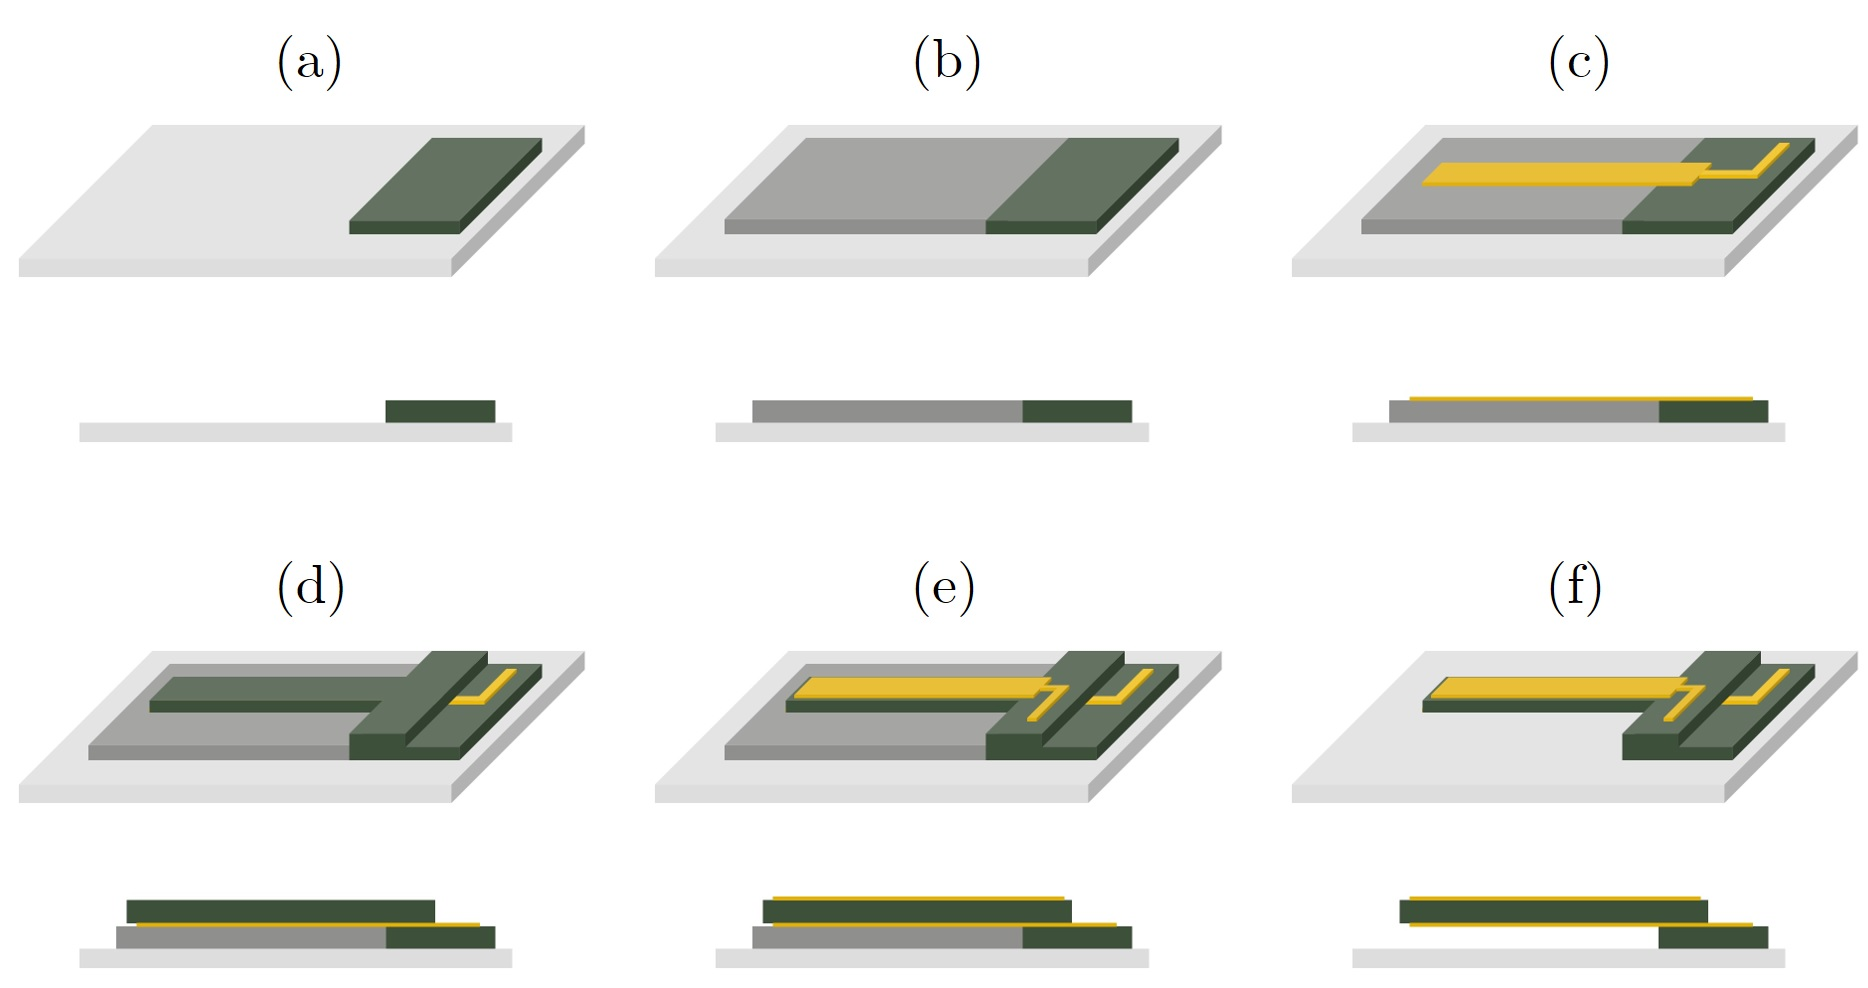
\includegraphics[width=\linewidth]{Images/full_proc}
%\end{figure}

\section{Agencement des couches et g�om�trie}
Les micropoutres r�sonnantes pr�sent�es ici sont fabriqu�es sur des substrats en alumine de 250 \textmu m d'�paisseur. La partie lib�r�e et le plot sont en zirco-titanate de plomb (PZT). Les �lectrodes prennent en sandwich la partie lib�r�e. Une couche sacrificielle soutient les �lectrodes et la partie lib�r�e jusqu'� l'�tape de frittage, durant laquelle la couche sacrificielle se d�compose. Plusieurs couches sacrificielles et �lectrodes sont test�es. Dans le proc�d� d�finit ici comme �standard�, les �lectrodes sont en or et la couche sacrificielle en polyester. L'empilement des couches est illustr� Figure \ref{empilement}. Des disques sont �galement fabriqu�s mais en moins grand nombre, avec un empilement identique mais sans plot, ce qui les lib�re donc totalement apr�s frittage. Ils servent de premier tests ou de r�f�rences dans les �volutions du proc�d�.\\

Diff�rentes g�om�tries de micropoutres sont test�es, faisant varier la longueur de la partie lib�r�e entre 8 mm et 1 mm et la largeur entre 2 mm et 1 mm (voir Tableau \ref{tab_geo}). � noter que dans la suite des travaux, la g�om�trie 8 mm de long pour 1 mm de large est abandonn�e, cassant trop souvent � la jonction plot-partie lib�r�e, probablement � cause de la masse importante et du rapport longueur/largeur trop fragilisant. Les �lectrodes font 0,2 mm de large de moins que la partie lib�r�e au niveau de cette derni�re  pour pr�venir les courts-circuits. Plus de d�tails sont donn�s sur les dimensions Figure \ref{empilement} \textbf{3}. Le dessin des �lectrodes a �galement �volu� pour s'adapter � l'ajout de modules de polarisation et d�acquisition utilisant des pointes de contact sur ressort. La Figure \ref{EI_ES} illustre cette �volution.\\


\begin{figure}
\centering
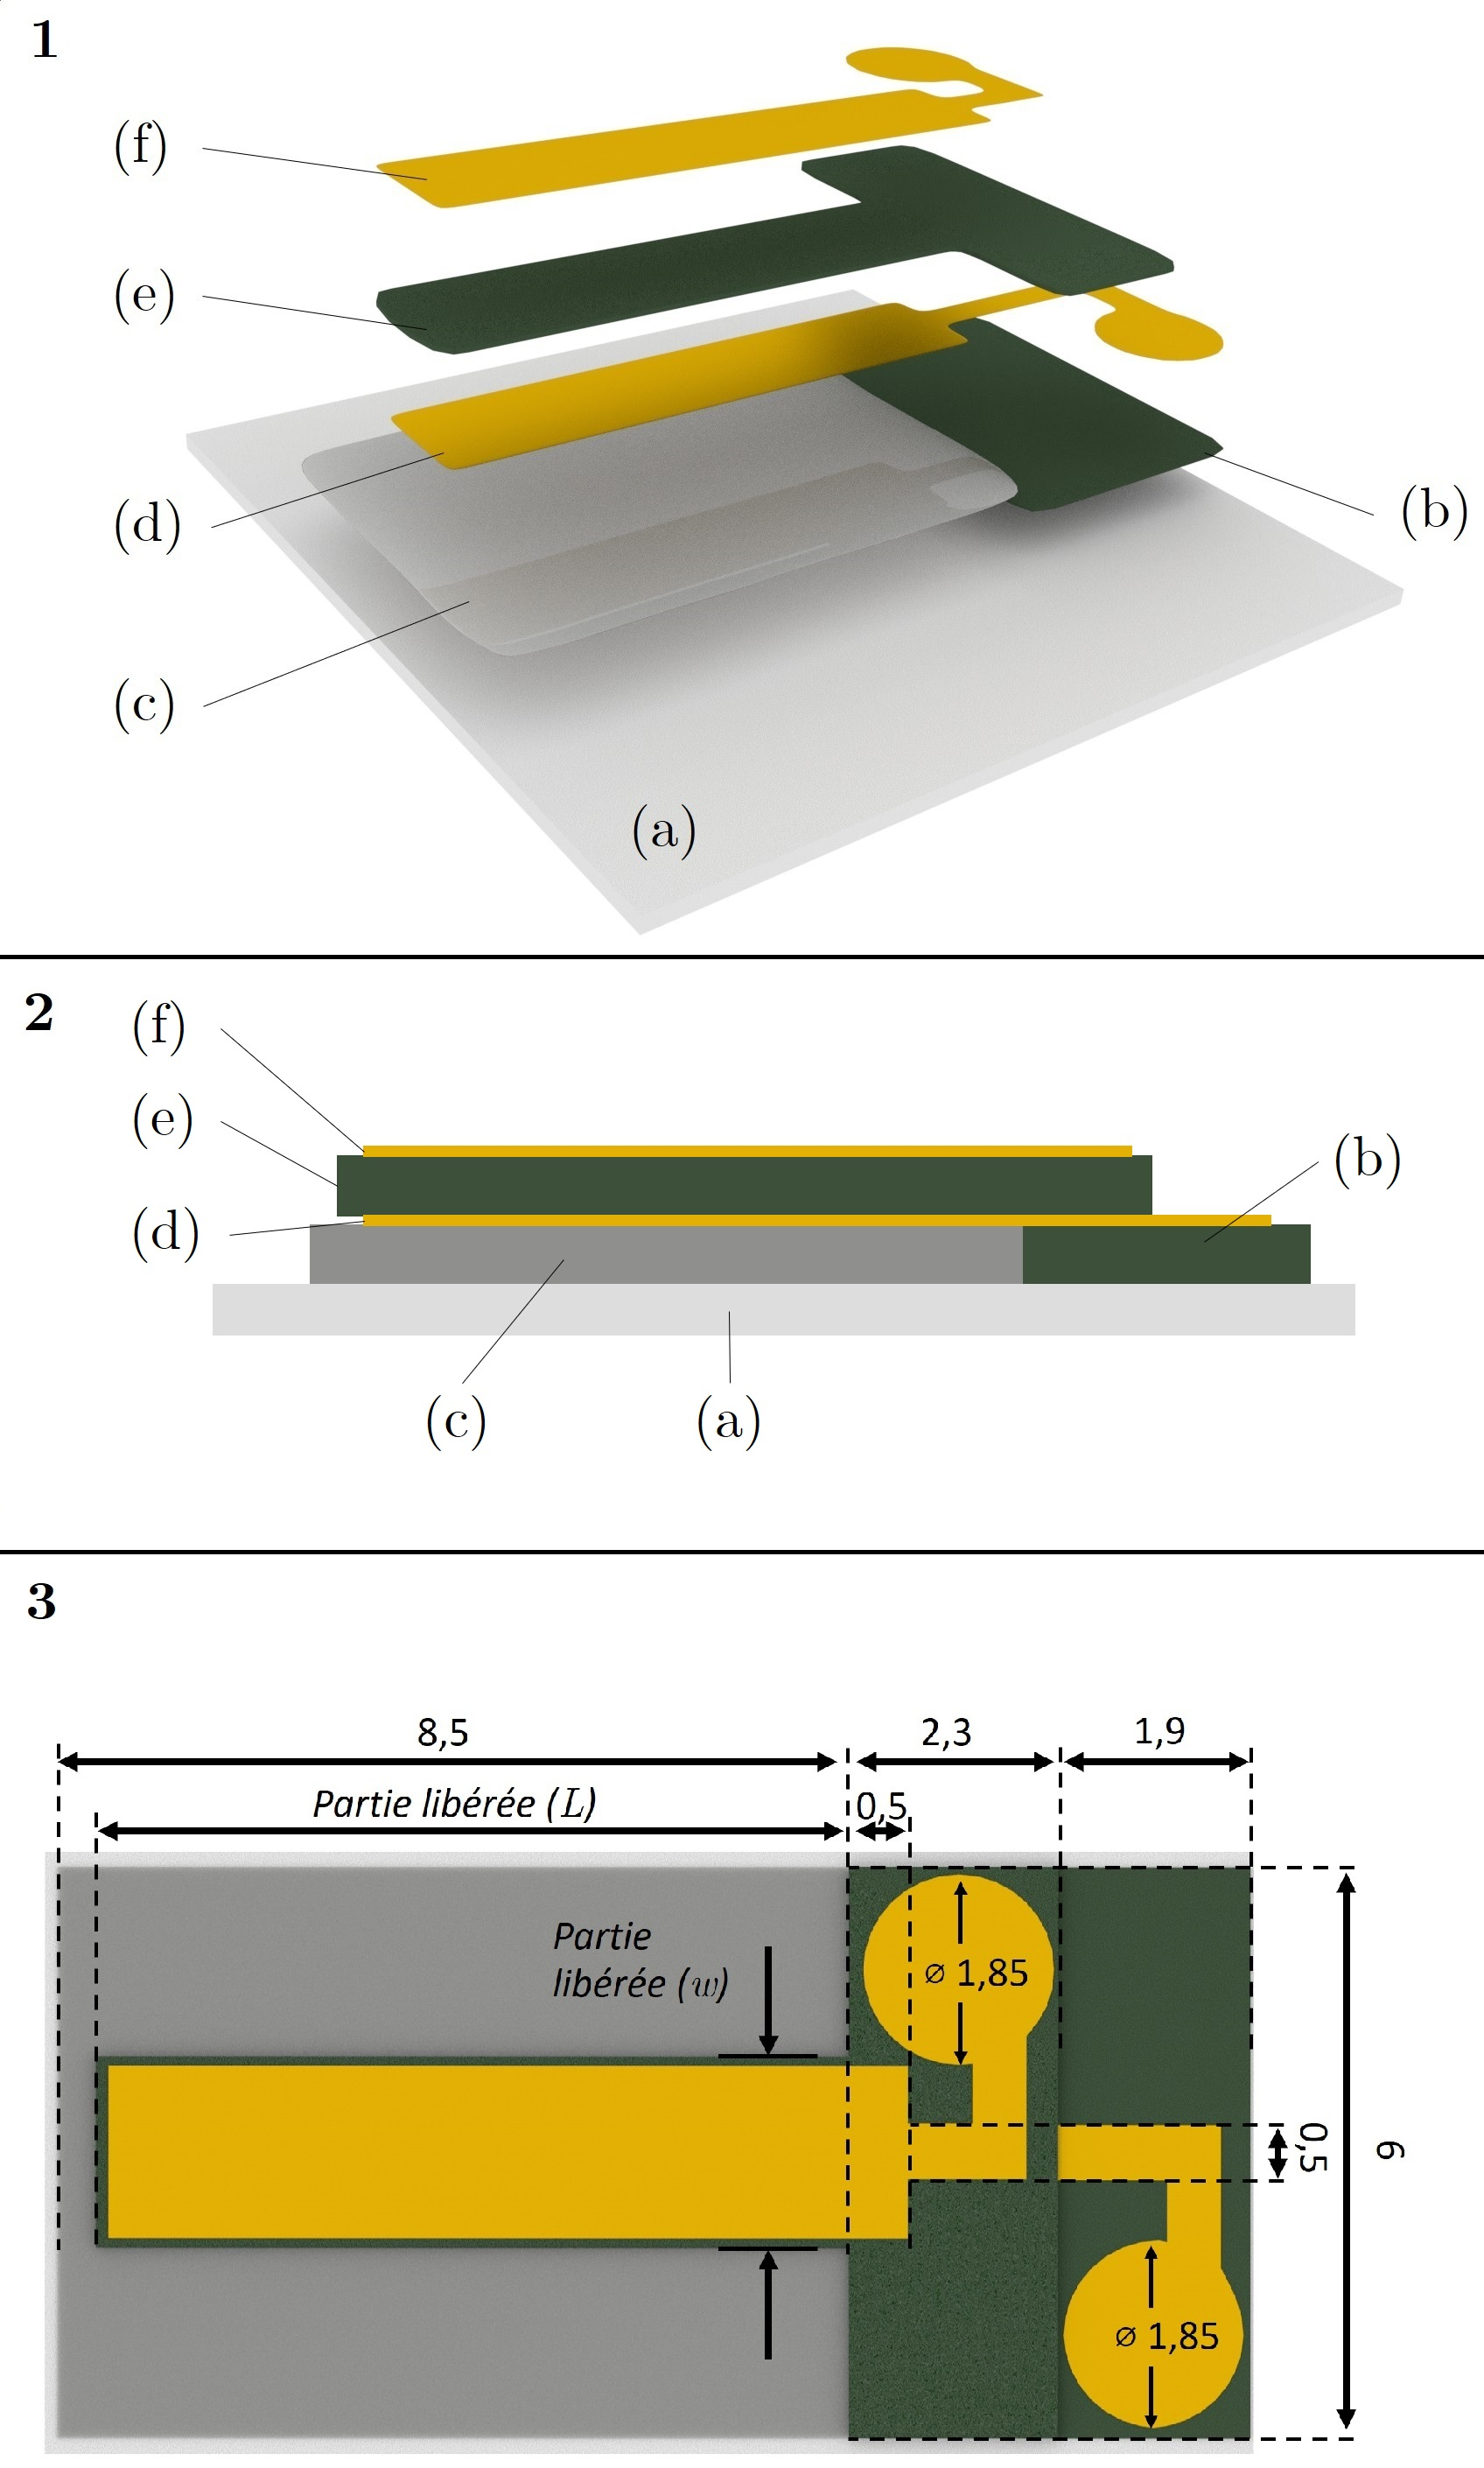
\includegraphics[width=0.70\linewidth]{Images/empilement}
\caption{\textbf{1} Vue �clat�e et \textbf{2} de profil de l'empilement des diff�rentes couches s�rigraphi�es pour une micropoutre de $8\times2\times0,1$ mm$^3$, avec (a) le substrat d'alumine, (b) le plot, (c) la couche sacrificielle, (d) l'�lectrode inf�rieure, (e) la partie lib�r�e et (f) l'�lectrode sup�rieure. \textbf{3} Vue de dessus avec les diff�rentes dimensions (\emph{L} et \emph{w} d'apr�s le Tableau \ref{tab_geo}).}
\label{empilement}%
\end{figure}

\begin{table}
\caption{Tableau r�sumant les longueurs (\emph{L}) et largeurs (\emph{w}) des diff�rentes micropoutres imprim�es. Les dimensions sont indiqu�es en millim�tres.}
\vspace{0.4cm}
\label{tab_geo}
\centering
\begin{tabular}{|c||c|c|c|c|c|c|c|c|}
\hline
\emph{L} 	&8&8&4&4&2&2&1&1\\ \hline 
\emph{w}		&2&1&2&1&2&1&2&1\\ \hline
\end{tabular}
\end{table}




\begin{figure}
\centering
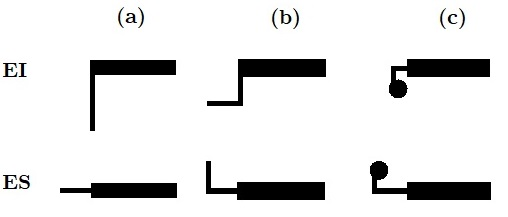
\includegraphics[scale=0.70]{Images/EI_ES}
\caption{Dessins de la (a) premi�re, (b) deuxi�me et (c) troisi�me g�n�ration d'�lectrodes utilis�es. \textbf{EI} $=$ �lectrode inf�rieure  \textbf{ES} $=$ �lectrode sup�rieure.}
\label{EI_ES}
\end{figure}



\section{La s�rigraphie}
\subsection{Principe g�n�ral}
La s�rigraphie consiste � faire passer, � l'aide d'une raclette, une encre � travers un �cran, ce dernier faisant office de pochoir pour le motif que l'on souhaite imprimer. L'empilement de diff�rents motifs et de diff�rentes couches permet la fabrication de dispositifs de nature et de tailles vari�es. Le principe d'impression par s�rigraphie est illustr� Figure \ref{serigraphie}.\\ 
Le proc�d� d'impression des diff�rentes couches se fait dans l'ordre indiqu� Tableau \ref{tab_fab}. Apr�s chaque impression, les couches sont s�ch�es � l'�tuve � 120�C pendant une dur�e variant de 20 min � plus d'une heure selon la couche. Ce tableau r�sume �galement les diff�rentes encres utilis�es ainsi que l'�paisseur apr�s �tuvage. Les d�tails concernant l'impression de chaque couche sont donn�s dans les sections suivantes. 

\begin{figure}
\centering
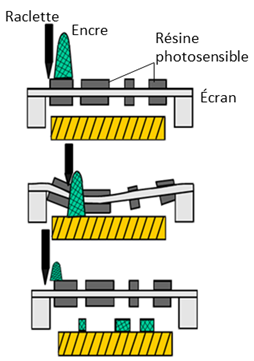
\includegraphics[width=0.3\linewidth]{Images/serigraphie}
\caption{Principe de l'impression par s�rigraphie.}
\label{serigraphie}%
\end{figure}

\begin{table}[h]
\caption{Tableau r�sumant la fabrication des micropoutres par s�rigraphie avec \emph{N} l'ordre d'impression. \emph{h} est l'�paisseur des couches apr�s �tuvage.}
\vspace{0.4cm}
\label{tab_fab}
\centering
\begin{tabular}{|c|c|c|c|c|}
\hline
\emph{N}&Couche 				&Encre							 &\emph{h} (\textmu m)		\\ \hline \hline 
1&Plot 						      &PZT								 &35		\\ \hline 
2&Couche sacrificielle	&ESL244T (polyester) &30		\\ \hline 
3&�lectrode inf�rieure	&ESL8836 (or)				 &15		\\ \hline 
4&Partie lib�r�e				&PZT								 &120	\\ \hline 
5&�lectrode sup�rieure 	&ESL8836 (or)				 &8		\\ \hline 
\end{tabular}
\end{table}


\subsection{�crans}
Les �crans de s�rigraphie utilis�s ici sont de deux types (voir �galement Figure \ref{mesh_vs_stencil}) :
\begin{itemize}
\item �crans mesh, constitu�s d'un maillage en acier et d'une couche de r�sine photosensible n�gative,
\item �crans en acier appel�s clinquants, dont le motif d'impression est d�coup� au laser.
\end{itemize}

\begin{figure}
\centering
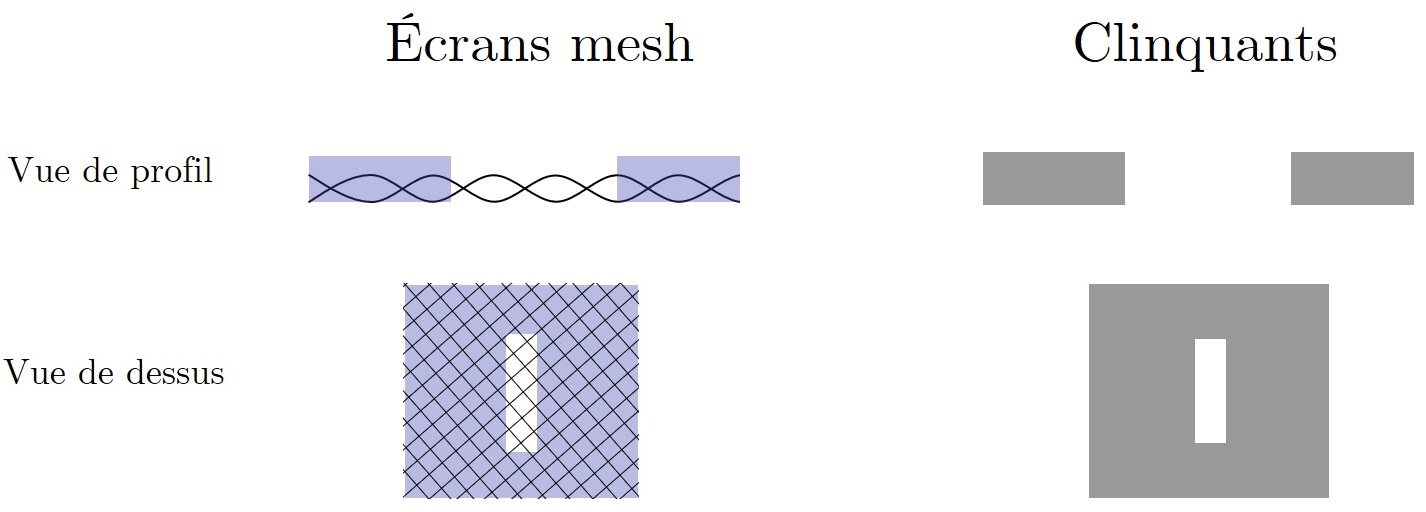
\includegraphics[width=0.8\linewidth]{images/mesh_vs_stencil.jpg}
\caption{Sch�ma de principe des �crans mesh et clinquants. Les �crans mesh sont constitu�s d'un maillage (ici en acier) et d'une r�sine photosensible dans laquelle est d�fini le motif � imprim� par insolation. Le maillage retient l'encre et la laisse passer lors du passage de la raclette. Les clinquants sont faits d'une seule feuille d'acier dans laquelle le motif est d�coup� au laser. }
\label{mesh_vs_stencil}
\end{figure} 

Les �crans mesh sont utilis�s pour toutes les couches imprim�es except�e la couche de PZT constituant la partie lib�r�e du dispositif final. Les diff�rents maillages utilis�s sont list�s dans le tableau \ref{tab_maill}.

\begin{table}[h]
\caption{Diff�rents �crans mesh utilis�s.\protect\footnote{Donn�es de la soci�t� DEK}}
\label{tab_maill}
\vspace{0.4cm}
\centering
\begin{tabular}{|c|c|c|c|c|c|} 
\hline
Nombre de	&\multirow{2}{*}{\o~fils (\textmu m)}	&Taille de 							&�paisseur 							&Tension			&Couche  \\
fils/pouce&																			&la maille (\textmu m)	&du maillage (\textmu m)&0,5\% (N/m)	&imprim�e	\\\hline\hline
70				&65																		&300										&$140\pm3$							&21-23 				&Co. sacri.\footnote{Couche sacrificielle} \\\hline
200				&36																		&90											&$80\pm2$								&20-22 				&Plot\\\hline
325				&24																		&53											&$52\pm1,5$							&13-15 				&EI et ES\footnote{�lectrodes inf�rieure et sup�rieure}\\\hline
400				&18																		&45											&$40\pm1$								&8-10  				&Mires\\\hline
\end{tabular}
\end{table}

Dans le reste de ces travaux, les �crans mesh sont d�sign�s par leurs nombre de fils par pouce : un �cran �70 mesh� d�signe par exemple l'�cran d�crit en premi�re ligne du Tableau~\ref{tab_maill}. Les maillages utilis�s vont du plus grossier (70 mesh) au plus fin (400 mesh). Un maillage fin offre une meilleur d�finition et une �paisseur plus fine, m�me si ces param�tres d�pendent aussi de l'�paisseur de la r�sine utilis�e. Une r�sine photosensible n�gative (VOIR NOM R�SINE) est appliqu�e sur les �crans, �paisse de 50 \textmu m sur les �crans 70 et 200 mesh, 15 \textmu m sur les autres. Cette r�sine est soluble dans l'eau avant insolation. La fixation sur les �crans se fait en exploitant cette propri�t�. Les �crans sont mouill�s de fa�on superficielle � l'aide d'un spray et la r�sine appliqu�e juste apr�s � l'aide d'une raclette. Ils sont ensuite s�ch�s � 60�C avant l'insolation aux UV avec le motif d�sir�.\\

Les clinquants sont constitu�s d'une feuille d'acier de 150 \textmu m d'�paisseur, dont les motifs sont d�coup�s au laser. Ils sont fournis par la soci�t� DB product. Le Tableau \ref{tab_fab_2} reprend le Tableau \ref{tab_fab} en y indiquant les �crans utilis�s dans la fabrication des micropoutres �tudi�es ici.\\

\begin{table}
\caption{Tableau r�sumant la fabrication des micropoutres par s�rigraphie avec \emph{N} = l'ordre d'impression. $h_{etu.}$ est l'�paisseur des couches apr�s �tuvage. Pour les �crans, la notation �200 mesh (50)� indique par exemple l'utilisation d'un �cran 200 mesh avec une r�sine photosensible de 50 \textmu m d'�paisseur.}
\vspace{0.4cm}
\label{tab_fab_2}
\centering
\begin{tabular}{|c|c|c|c|c|}
\hline
\emph{N}&Couche 				&Encre							 &$h_{etu.}$ (\textmu m)&�cran				\\ \hline \hline 
1&Plot 						      &PZT								 &30-40									&200 mesh (50)\\ \hline 
2&Couche sacrificielle	&ESL244T (polyester) &30-40									&70 mesh (50)	\\ \hline 
3&�lectrode inf�rieure	&ESL8836 (or)				 &15										&325 mesh (15)\\ \hline 
4&Partie lib�r�e				&PZT								 &100-120								&Clinquant		\\ \hline 
5&�lectrode sup�rieure 	&ESL8836 (or)				 &8											&325 mesh (15)\\ \hline 
\end{tabular}
\end{table}

Les �crans mesh permettent la d�position de formes vari�es et de couches de diff�rentes �paisseurs  en fonction de la r�sine et du maillage utilis�. Plus le maillage est fin, plus le motif sera pr�cis et la couche fine. Un espace entre le substrat et l'�cran (�hors contact�) est n�cessaire � l'impression, l'�cran se d�formant et n'�tant en contact avec le substrat qu'au passage de la raclette (voir Figure \ref{gap}).
L'impression avec des clinquants en acier se fait sans hors contact. Ils permettent une impression aux motifs plus pr�cis et plus �pais (>100 \textmu m), mais l'impression de couches fines est impossible en raison de la fragilit� des feuilles d'acier � partir de 100 \textmu m d'�paisseur.

\begin{figure}
\centering

\includegraphics[width=0.8\linewidth]{images/gap2.jpg}
\caption{Illustration d'une impression avec un �cran mesh. Apr�s le passage de la raclette, l'�lasticit� de l'�cran le d�colle du substrat.}
\label{gap}
\end{figure} 

\subsection{S�rigraphieuse � param�tres critiques}
La s�rigraphieuse utilis�e est une DEK Horizon (entreprise MJB), comportant notamment un syst�me de lecture de mires et d'alignement automatis�. Une photo de la DEK est visible Figure (PHOTO DECK). Des raclettes avec un angle d'attaque de 45� sont utilis�e, en polyur�thane sur les �crans mesh et en acier pour les clinquants.
\label{shim}
\paragraph{Shims}
Les substrats sont d�pos�s sur une table de s�rigraphie aspirante pour les emp�cher de bouger. Les shims sont des feuilles d'acier trou�es � la forme du substrat, d'�paisseurs calibr�es et qui permettent l'ajustement de la hauteur de la table de s�rigraphie au substrat et aux couches imprim�es. Par exemple, si on utilise un substrat d'alumine de 250 \textmu m, on devra utiliser un shim de la m�me �paisseur. Dans le cas pr�sent pour l'�lectrode sup�rieure, on utilise un shim de 400 \textmu m, car elle est imprim�e sur alumine (250 \textmu m) + couche sacrificielle/plot ($\approx$35 \textmu m) + �lectrode inf�rieure (15 \textmu m) + partie lib�r�e (100 \textmu m) $\approx$ 400 \textmu m. On consid�re qu'en dessous de 50 \textmu m d'�cart entre la hauteur n�cessaire et le shim, il n'est pas indispensable de le changer.\\
La hauteur des shims a un impact important sur l'�paisseur des couches s�rigraphi�es. Un shim trop �pais augmentera l'�paisseur imprim�e, un  trop fin peut endommager l'�cran qui sera en contact avec une zone �ventuellement non plane autour de la zone � imprimer.
\paragraph{Alignement et mires}
L'alignement des motifs est automatis� sur la s�rigraphieuse utilis�e via la reconnaissance vid�o de mires. Ces mires sont incorpor�es aux motifs des �crans et bouch�es avec de la laque d'argent pour faciliter leur reconnaissance. Les mires sont �galement imprim�es sur des substrats vierges avec un �cran 400 mesh et une �mulsion de 15\textmu m d'�paisseur avant le d�but de la fabrication des micropoutres dans une encre di�lectrique fritt�e � 850�C. Cependant, il a �t� remarqu� � plusieurs reprise de l�g�res impr�cisions qui n�cessitent de v�rifier l'alignement r�guli�rement sous peine de voir un d�calage appara�tre entre les couches imprim�es successivement.
\paragraph{Pression de la raclette sur les �crans}
Pour les raclettes en polyur�thane, l'usure est plus rapide que pour les raclettes en acier (usure non observ�e sur la dur�e de ces travaux), d'autant plus avec un mauvais param�trage de l'impression, comme par exemple une pression de la raclette sur les �crans trop importante. Cela a pour effet d'user pr�matur�ment les �crans mesh et surtout de changer l'angle d'attaque de la raclette, ce qui peut emp�cher le passage de l'encre � travers l'�cran.
\paragraph{Vitesse d'impression}
La vitesse d'impression doit �tre adapt�e � la viscosit� de chaque encre. Plus une encre est visqueuse, plus la vitesse doit �tre �lev�e.
\paragraph{Vitesse de s�paration}
Il s'agit de la vitesse � laquelle le substrat est �loign� de l'�cran apr�s impression. Ceci est plut�t une cons�quence de la distance de hors contact pour les �crans mesh, mais peut poser probl�me dans le cas des clinquants o� une vitesse trop faible pourra laisser des bavures sur les contours des motifs.
\paragraph{Ordre et direction de l'impression}
L'impression des motifs doit autant que possible se faire dans le sens de la plus grande longueur des motifs. Si deux couches sont imprim�es l'une � c�t� de l'autre, l'ordre d'impression reste a prendre en compte : cela impacte la forme de la jonction, comme par exemple quelle couche recouvrira partiellement l'autre � cet endroit. La direction d'impression change �galement la forme de la jonction. Imprimer d'une couche haute vers une couche basse a tendance � cr�er des espaces (�gap�) � la jonction. � l'inverse des recouvrements plus ou moins importants se font lors de l'impression d'une couche basse vers une couche haute. Une impression lat�rale peut permettre une jonction parfaitement ajust�e �vitant les deux d�fauts, mais n�cessite une plus grande pr�cision si l'on veut assurer un gap ou un recouvrement syst�matique. En g�n�ral g�n�ral l'un ou l'autre des d�fauts est plus critique. On pr�f�rera un faible recouvrement de deux couches vou�es � �tre recouverte par une troisi�me couche plut�t qu'un gap compromettant potentiellement l'int�grit� de cette derni�re. On pr�f�rera � l'inverse un gap plus grand que pr�vu entre deux couches conductrices si elles ne doivent pas �tre connect�es.

Les param�tres d'impression de chaque couche sont fournis en (ANNEXE).

%\begin{figure}
%
%\includegraphics{lol}
%\caption{}
%\label{serigraphieuse}
%\end{figure} 

\subsection{Encres de s�rigraphie}
Les encres de s�rigraphie doivent avoir un comportement rh�ofluidifiant, i.e. dont la viscosit� diminue quand le taux de cisaillement augmente \cite{Lin2008}. Cela permet la tenue des encres au repos dans les mailles des �crans mesh et apr�s impression, mais aussi le passage de l'encre � travers les �crans lors du cisaillement impos� au passage de la raclette.\\
On peut s�par� les composants d'une encre de s�rigraphie en 3 cat�gories :
\begin{itemize}
\item La charge active, qui donne ses propri�t�s d'int�r�t � la couche (conductivit�, r�sistance en temp�rature, di�lectricit�, flexibilit�, pi�zo�lectricit�). Elle peut �tre faite d'un m�lange de poudres, de polym�res ou d'un m�lange de monom�res.
\item Le solvant, qui permet la mise en encre de la charge sous forme de p�te.
\item Le liant organique, qui sert � maintenir la couche en forme apr�s impression et �vaporation du solvant comme par exemple l'�thylcellulose.
\end{itemize}
Dans le cadre de la formulation d'encres, le solvant et le liant sont parfois vendus ensemble d�j� m�lang�s sous le nom de �v�hicule organique�. C'est le cas dans ces travaux pour les encres fabriqu�es au sein du laboratoire. Les diff�rents types d'encres utilis�s sont d�crits dans les sections suivantes.


\section{Couches sacrificielles}

Au cours de ces travaux, plusieurs encres de s�rigraphie ont �t� test� comme couche sacrificielle et sont d�crites dans les sous-parties suivantes. Lors de la fabrication, les couches sont toutes s�ch�es � l'�tuve � 120�C pendant 20 minutes apr�s avoir �t� s�rigraphi�es (sauf mention contraire explicite), permettant l'�vaporation des solvants.

\subsection{\texorpdfstring{Carbonate de strontium (SrCO$_3$)}{Carbonate de strontium (SrCO3)}}
La couche sacrificielle � base de carbonate de strontium (SrCO$_3$) a �t� d�velopp�e au cours de travaux pr�c�dents dans le Laboratoire IMS \cite{Lucat2008,Lakhmi2014}. Elle est compos�e d'une base min�rale de carbonate de strontium et d'un v�hicule organique � base de r�sine �poxy (�lectroScience ESL CV59), qui contient un solvant (ac�tate de butyl diglycol), un pr�polym�re (�ther de bisph�nol A diglycidylique) et un durcisseur, catalyseur de la r�action de polym�risation de type anhydride d'acide (voir Tableau \ref{srco3}). L�int�r�t est que si la d�composition se d�roule � environ 275�C pour la r�sine �poxy, la partie min�rale reste stable jusqu'� environ 1100�C et peut donc servir de support m�canique pendant le frittage des autres couches qui a lieu � 900�C. La partie min�rale restante est ensuite  retir�e par voie humide, via la r�action suivante :
\begin{center}
	$SrCO_{3_{(Solide)}} + 2H_3O^+ \Leftrightarrow CO_{2_{(Gaz)}} + Sr^{2+} + H_2O$
\end{center}
Concr�tement, cette derni�re op�ration se fait dans une solution � 0,5 mol.$^{-1}$ d'acide phosphorique. Cette �tape prend n�anmoins du temps et est une source possible de d�gradation des syst�mes lib�r�s de part les manipulations requises.
La couche est s�rigraphi�e en une fois, pour une �paisseur s�che d'environ 35 \textmu m.
	
	
\begin{table}
\caption{Composition de l'encre SrCO$_3$ (d'apr�s \cite{GINET2013})}
\label{srco3}
\vspace{0.4cm}
\centering
\begin{tabular}{|c|c|}
\hline
Partie min�rale									&V�hicule organique (ESL CV59)\\\hline\hline
\multirow{3}{*}{SrCO$_3$}				&Ac�tate de Butyl Diglycol \hfill+\\
																&�ther de bisph�nol A diglycidylique \hfill+\\
																&Anhydride d'acide (non-sp�cifi�)\hfill~\\\hline
\end{tabular}
\end{table}
%\end{tabular}
%
%\end{table}
%
%\begin{table}
%\caption{Composition de l'encre SrCO$_3$}
%\label{srco3}
%\vspace{0.4cm}
%\centering
%\begin{tabular}{|c|c|c|}
%\hline
%\multirow{2}{*}{Partie min�rale}& \multicolumn{2}{c|}{V�hicule organique}\\\cline{2-3}
																%& Solvant		& 							Liant			\\\hline\hline
%SrCO$_3$&Ac�tate de Butyl Diglycol&
%\end{tabular}
%
%\end{table}	
	
\subsection{Polyester (ESL 244t)}
Il s'agit de l'encre majoritairement utilis�e dans ces travaux. L'encre commerciale ESL 244t (par la suite abr�g�e en � 244t �) est une encre fabriqu�e par ESL ElectroScience comme couche de protection contre l'humidit�. Les informations du fabriquant indiquent un m�lange de polym�re de type polyester avec un solvant organique (ac�tate de butyle diglycol). L�int�r�t d'une encre sans composant min�ral est que l'on peut s'abstenir de l'�tape de retrait : la 244t se d�compose int�gralement entre 250�C et 450�C. L'absence de couche sous jacente pour �retenir� les couches support�es par la couche sacrificielle peut aussi permettre une meilleure densification lors du frittage.\\
La 244t est s�rigraphi�e en deux fois, pour une �paisseur s�che d'environ 30 � 40 \textmu m en fonction des lots. Un premier s�chage � 120�C pendant 20 minutes � lieu entre les deux d�p�ts, un second ensuite � la m�me temp�rature pendant cette fois-ci 30 minutes. � la diff�rence de la r�sine �poxy utilis�e dans l'encre SrCO$_3$, le s�chage est en r�alit� une polym�risation des monom�res pr�curseurs du polyester. Le second s�chage plus long permet de s'assurer de cette derni�re.\\
La 244t pr�sente un certain vieillissement en pot, � cause de l'�vaporation progressive des solvants. Ceci a tendance � augmenter la  viscosit� au cours du temps et permet alors une impression de 30 \textmu m d'�paisseur en une fois. Cet aspect �tant difficile � contr�ler, il reste pr�f�rable d'utiliser une encre neuve et d'effectuer l'impression en 2 fois. 
	
\subsection{Exp�rimentation : � base de ma�s}
Cette section rassemble les r�sultats obtenus lors d'exp�rimentations faites avec une couche sacrificielle � base de farine de ma�s, en parall�le de la fabrication de micropoutres sur 244t, standard dans le reste de ces travaux.\\ 

L'encre est compos�e d'un v�hicule � base de r�sine �poxy (ESL CV59) et de farine de ma�s industrielle. Un m�lange dans les proportions 30 wt\% v�hicule/70~wt\% poudre est d'abord r�alis� au pilon et au mortier, avant une homog�n�isation dans un m�langeur tri-cylindre. Ce m�lange est successivement dilu� avec le v�hicule ESL CV59. Chaque composition est ensuite test�e sur la s�rigraphieuse, jusqu'au succ�s du d�p�t. Les r�sultats sont r�sum�s dans le tableau \ref{tab_mais}.

\begin{table}
\caption{R�sum� des r�sultats des dilutions lors de l'�laboration de l'encre � base de farine de ma�s}
\label{tab_mais}
\vspace{0.4cm}
\centering
\begin{tabular}{|c|c|c|c|}
\hline
wt \% de v�hicule	& S�rigraphiable \\
\hline \hline
30&Non\\\hline
32&Non\\\hline
34&Non\\\hline
36&Oui\\\hline
\end{tabular}

\end{table}

La composition 36wt \% v�hicule/64wt \% poudre se montre s�rigraphiable, avec une �paisseur apr�s s�chage d'environ 100 \textmu m. En raison d'un manque de disponibilit� imm�diate des mat�riaux, et ces travaux  n'�tant pas consacr�s � l'�laboration d'une nouvelle encre de s�rigraphie, une seule s�rie de micropoutres et deux disques de PZT sont fabriqu�s avec cette couche sacrificielle. La totalit� des micropoutres est lib�r�e lors du frittage, mais la plupart pr�sente des d�fauts les rendant non-exploitables :
\nopagebreak
\begin{itemize}
\item fissures � l'encastrement
\item �lectrode coup�e/sous-imprim�e
\end{itemize}
Ces d�fauts sont tr�s probablement dus � l'�cart entre le niveau du plot (35 \textmu m) et la couche sacrificielle (100 \textmu m). Ce probl�me, �galement rencontr� avec la 244t, est plus amplement trait� dans la section \ref{pb_gap}. Malgr� ces d�fauts, une micropoutre est polaris�e et pr�sente des pics de r�sonances compatibles avec les fr�quences attendues en th�orie. Les disques sont �galement lib�r�s et la couche de PZT pr�sente une densit� sensiblement plus �lev�e que dans les micropoutres (voir section \ref{carac} pour les caract�risations m�caniques).

\section{Encre PZT}

\subsection{Composition}
L'encre PZT qui constitue le plot et la partie lib�r�e des micropoutres est fabriqu�e au sein du laboratoire IMS. Elle est compos�e d'un v�hicule organique (ESL V400) et d'une partie min�rale. Le v�hicule organique (solvant de type alcool-ester + liant ethylcellulose) permet la mise en encre et la tenue apr�s s�chage et jusqu'au frittage. La partie min�rale est un m�lange de poudres de zirco-titanate de plomb PbZr$_{0.52}$Ti$_{0.48}$O$_3$ (Pz26, Ferroperm) et de LBCu (Li$_2$CO$_3$, Bi$_2$O$_3$, CuO Sigma Aldrish). C'est un additif d'aide au frittage utilis� pour diminuer la temp�rature de frittage du PZT \cite{Medesi2014,Lakhmi2011}. La composition utilis�e dans ces travaux est r�sum�e dans le Tableau \ref{compo_PZT}.\\
Les poudres composantes du LBCu sont broy�es dans un broyeur plan�taire avec de l'�thanol et des billes de zircon pendant 12h. Apr�s s�chage les poudres de PZT, Li$_2$CO$_3$, Bi$_2$O$_3$ et CuO sont pes�es puis m�lang�es au m�langeur plan�taire dans un flacon contenant 8 billes en agate et 40 ml d'�thanol pendant une nuit. Apr�s s�chage, le v�hicule et la poudre sont m�lang�s au mortier puis dans un m�langeur tri-cylindre, qui permet de cisailler l'encre, cassant les agglom�rats et homog�n�isant le m�lange. La proportion v�hicule/poudre est discut�e dans le paragraphe suivant.

\begin{table}
\caption{Composition de la partie min�rale de l'encre PZT.}
\label{compo_PZT}
\vspace{0.4cm}
\centering
\begin{tabular}{|c|r|}
\hline
Poudre	& wt \% \\
\hline \hline
PbZr$_{0.52}$Ti$_{0.48}$O$_3$ &97,00\\\hline
Li$_2$CO$_3$&0,80\\\hline
Bi$_2$O$_3$&1,20\\\hline
CuO&1,00\\\hline
\end{tabular}

\end{table}

\subsection{Optimisations}
\subsubsection{Encres mesh et clinquant}
Deux proportions diff�rentes de v�hicule sont utilis�es pour les �crans mesh et les clinquants. Il est avantageux d'avoir une encre assez fluide pour un �cran mesh, o� il est pr�f�rable que l'encre �lisse� apr�s impression pour att�nuer la marque laiss�e par les mailles. Une encre plus visqueuse permet en revanche une meilleure tenue du motif avec un clinquant, o� l'encre n'est pas soutenue par un maillage et le d�p�t est plus �pais. Une plus faible proportion de v�hicule est �galement souhaitable pour le s�chage de couches �paisses afin d'�viter les fissures dues � l'�vaporation du solvant. De plus aucun lissage post-impression n'est n�cessaire. (PHOTOS) Les proportions optimales sont obtenues par essais successifs � la s�rigraphieuse jusqu'� l'obtention de l'aspect d�sir�. Les compositions  finales utilis�es sont indiqu�es dans le Tableau \ref{compo_PZT2}. Les �carts indiqu�s correspondent aux �carts aux valeurs cibles obtenus lors des pes�es.\\
La viscosit� des encres a �t� mesur�e � 25�C � l'aide d'un rh�om�tre plan-plan On peut voir sur la Figure \ref{viscosity_PZT} que les encres ont un comportement rh�ofluidifiant, comme attendu pour des encres de s�rigraphie. On note �galement la viscosit� plus importante de l'encre destin�e aux clinquants.
\begin{table}
\caption{Proportions poudre/v�hicule organique de l'encre PZT. Une encre est �labor�e pour les impressions faites avec un �cran mesh et une autre pour les impressions avec les clinquants.}
\label{compo_PZT2}
\vspace{0.4cm}
\centering
\begin{tabular}{|c|c|c|}
\hline
Type d'�cran&PZT+LBCu (wt \%)&ESL V400 (wt \%)\\\hline \hline
Clinquants&85,7$\pm$0,2											&	14,3$\pm$0,2\\\hline
Mesh			&84,1$\pm$0,3											&15,9$\pm$0,3\\\hline
\end{tabular}
\end{table}



\begin{figure}
\centering
\begin{tikzpicture}
\begin{axis}[
  xlabel=Taux de cisaillement (s$^{-1}$),
  ylabel=Viscosit� (Pa.s),
	minor xtick={0,25,...,200},
	minor ytick={0,50,...,400},
	grid=major,
	legend cell align={left}]
%\draw[step=1cm,gray,very thin] (-2,-2) grid (6,6);	
\addplot table [y=EncrePZTmesh, x=Tauxdecisaillement]{Images/viscosity_PZT.dat};
\addlegendentry{Encre PZT mesh}
\addplot table [y=EncrePZTclinquant, x=Tauxdecisaillement]{Images/viscosity_PZT.dat};
\addlegendentry{Encre PZT clinquant}
\end{axis}
\end{tikzpicture}
\caption{Viscosit�s des encres PZT (non-broy�) pour les �crans mesh et clinquant. Mesure effectu�e � 25�C avec un rh�om�tre plan-plan.}
\label{viscosity_PZT}
\end{figure}

\subsubsection{Encre PZT broy�}
Dans les compositions pr�c�dentes, seul les poudres de l'aide au frittage LBCu sont broy�es. La poudre PZT est � son tour broy�e selon le m�me proc�d� et ceci dans l'espoir d'am�liorer les propri�t�s m�caniques en favorisant un meilleur frittage et une plus faible porosit� avec la diminution de la taille des grains. La diminution de la taille des grains a pour cons�quence d'augmenter la surface totale de la poudre, rendant n�cessaire l'adaptation des proportions poudre/v�hicule. Si l'encre est d'abord d�velopp�e pour les clinquants, la composition utilis�e s'est r�v�l�e �galement bonne pour les �crans mesh. Un ratio 14,9$\pm$0,1 wt\% de v�hicule pour 85,1$\pm$0,1 wt\% de poudres PZT+LBCu permet une s�rigraphie satisfaisante sur �crans mesh et clinquants. Aucune diff�rence notable d'�paisseur n'est observ�e apr�s �tuvage entre les encres PZT broy� et non-broy�.

\subsubsection{Am�liorations ult�rieures possibles}
Les encres PZT �labor�es sont r�alis�es empiriquement par essais successifs � la s�rigraphieuse pour chaque proportion poudre/v�hicule. De plus, les compositions massiques sont retenues pour la reproductibilit� des encres, alors que le param�tre clef pour la s�rigraphie est la viscosit� \cite{Lin2008, Reinhardt2018}, qui peut d�pendre de la temp�rature de formulation. Il serait plus efficace et exact de pr�parer les encres en v�rifiant �galement la  viscosit� et la temp�rature durant la mise en encre (avec le v�hicule organique) et l'impression, avec par exemple un viscosim�tre portable. 

\subsection{Impressions plot et partie lib�r�e}
\subsubsection{Proc�d� classique}
Le plot est imprim� avec un �cran 200 mesh et une r�sine photosensible de 50 \textmu m d'�paisseur. Le d�p�t se fait en une fois sur un substrat d'alumine et est s�ch� 20 minutes � l'�tuve, pour une �paisseur s�che de 30 � 40 \textmu m en fonction des lots.\\
La partie lib�r�e recouvre en partie le plot et l'�lectrode inf�rieure. Elle est imprim�e avec un clinquant de 150 \textmu m d'�paisseur en une fois. Du fait de son �paisseur, et pour �viter les fissures, la couche est s�ch�e dans une �tuve programmable avec un gradient de 1�C/min jusqu'� 120�C, puis maintenue � temp�rature pendant une heure. L��paisseur s�che est d'environ 100 \textmu m.

\subsubsection{Variation d'�paisseur de la partie lib�r�e}
En utilisant un clinquant de 150 \textmu m, il est possible d'imprimer des couches de plus de 150 \textmu m d'�paisseur apr�s �tuvage en changeant le shim utilis� (plus de d�tails sur les shims section \ref{shim}). Un lot est imprim� ainsi. On obtient g�n�ralement de meilleures propri�t�s m�caniques et des r�sonances de meilleure qualit�. Mais ces am�liorations apparentes se font au prix d'une augmentation non n�gligeable de la masse. Or la sensibilit� d'un r�sonateur utilis� comme capteur gravim�trique est d�finie de la fa�on suivante :
\begin{center}
$S=\frac{-f_0}{2m}$
\end{center}
avec $S$ la sensibilit� th�orique, $f_0$ la fr�quence de r�sonance et $m$ la masse du capteur.\\
Il appara�t alors de fa�on �vidente qu'une augmentation de la masse entra�ne une diminution de la sensibilit�. Il est difficile d�s lors de trancher entre les b�n�fices apport�s par l'am�lioration des propri�t�s m�caniques et la diminution de la sensibilit� th�orique. Il semble pr�f�rable n�anmoins de rechercher les possibilit�s d'impression de parties lib�r�es plus fines tout en conservant les meilleures propri�t�s m�caniques possibles.\\

Dans cette optique un clinquant de 100 \textmu m d'�paisseur est utilis� pour la fabrication de parties lib�r�e plus fines entre 90 et 70 \textmu m d'�paisseur apr�s �tuvage. D'un point de vue proc�d�, le probl�me d'une partie lib�r�e plus fine est de fa�on assez �vidente sa fragilit� augment�e. Deux lots de 16 micropoutres chacun sont cependant imprim�s et fritt�s avec succ�s avec l'encre de PZT broy�.\\



 
\section{�lectrodes}
\label{compat_solvants}
\subsection{Encre � base d'or}
Une encre � base d'or et de terpin�ol (�lectroscience ESL 8836) est utilis�e pour les �lectrodes. Une fritte de verre est incluse dans la composition et permet la bonne adh�sion entre or et PZT apr�s le frittage. Les �lectrodes sont imprim�es avec un �cran 325 mesh et une r�sine photosensible de 15 \textmu m d'�paisseur. L'�lectrode inf�rieure est imprim�e en deux fois pour une �paisseur s�che de 15 \textmu m, et l'�lectrode sup�rieure est imprim�e en une fois, pour une �paisseur s�che de 8 \textmu m. Le choix de cette dissym�trie a pour origine une interaction entre solvants discut�e section \ref{inter_solvants}. 

\subsection{Encre � base d'argent}
\label{AgPd}
ATTENTE D�TAILS TEMEX
\subsubsection{Composition}
Une encre conductrice � base d'argent-palladium (Ag 90wt\%/Pd 10 wt\%) fournie par l'entreprise TEMEX est test�e comme alternative � l'encre en or. L'argent pr�sente en outre l�int�r�t d'�tre moins cher et compatible avec des alliages de soudures beaucoup moins co�teux que pour l'or (BIBLIO). Compos�e de () et de (), l'encre est imprim�e avec le m�me �cran que pour l'or (325 mesh + 15 \textmu m de r�sine). Dans un premier temps, des couches simples sont s�rigraphi�es pour les �lectrodes inf�rieure et sup�rieures.Les couches sont plus fines que celles imprim�es avec l'or dans les m�me conditions, et on observe des discontinuit�s de l'�lectrode au microscope �lectronique (voir Figure \ref{agpd_thin}). Le doublage des deux �lectrodes r�sout le probl�me, pour une �paisseur apr�s �tuvage de 10 \textmu m chacune. (Tableau compo)\\

Autre encre avec partie min�rale adapt�e pour �viter les fissures?


\begin{figure}
\centering

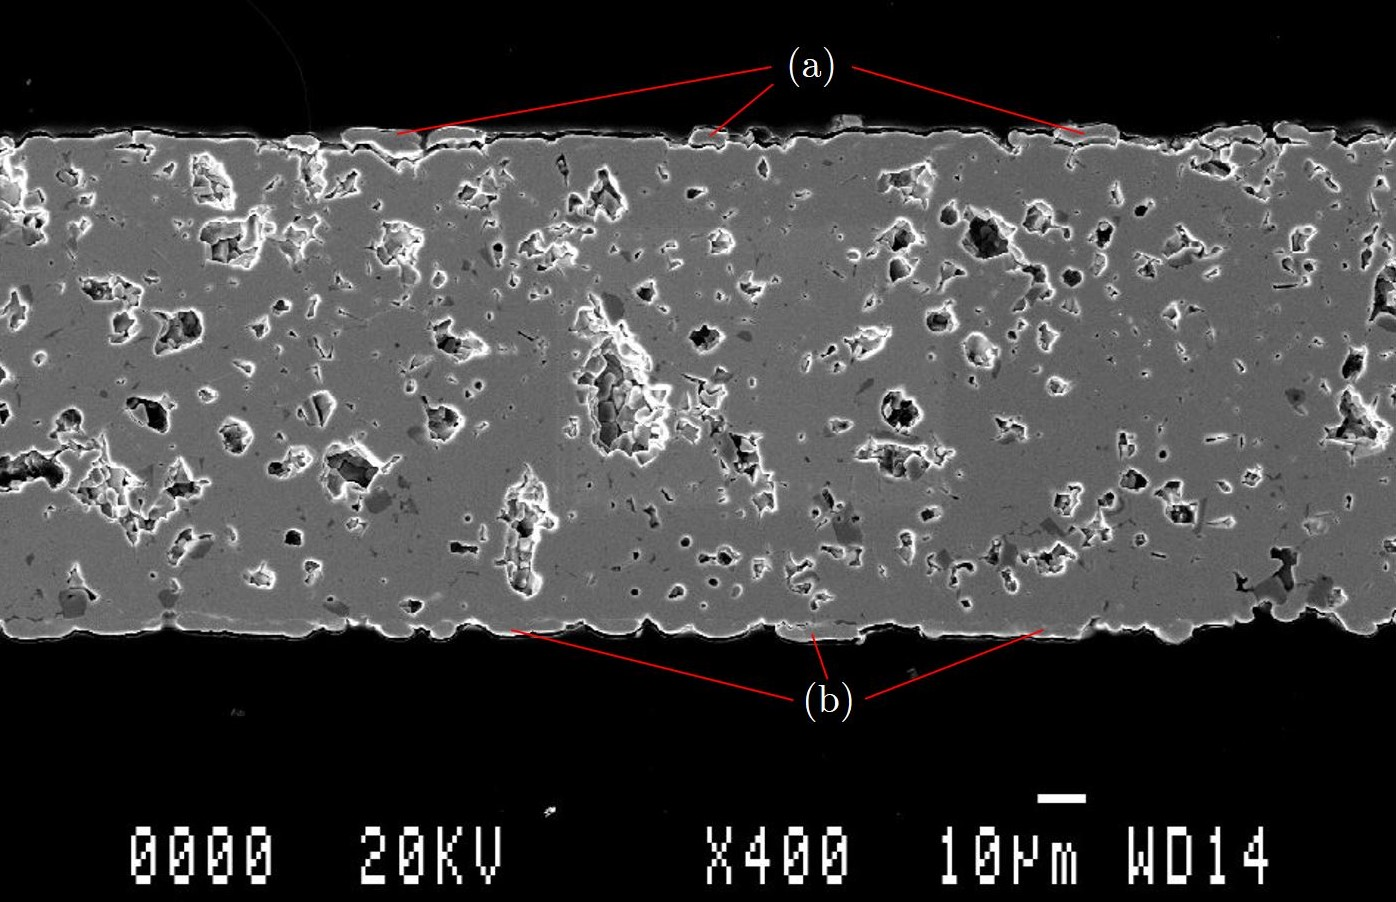
\includegraphics[width=0.6\linewidth]{Images/agpd_thin_note.jpg}
\caption{Simple couche d'argent.}
\label{agpd_thin}

%\begin{subfigure}{0.6\textwidth}
%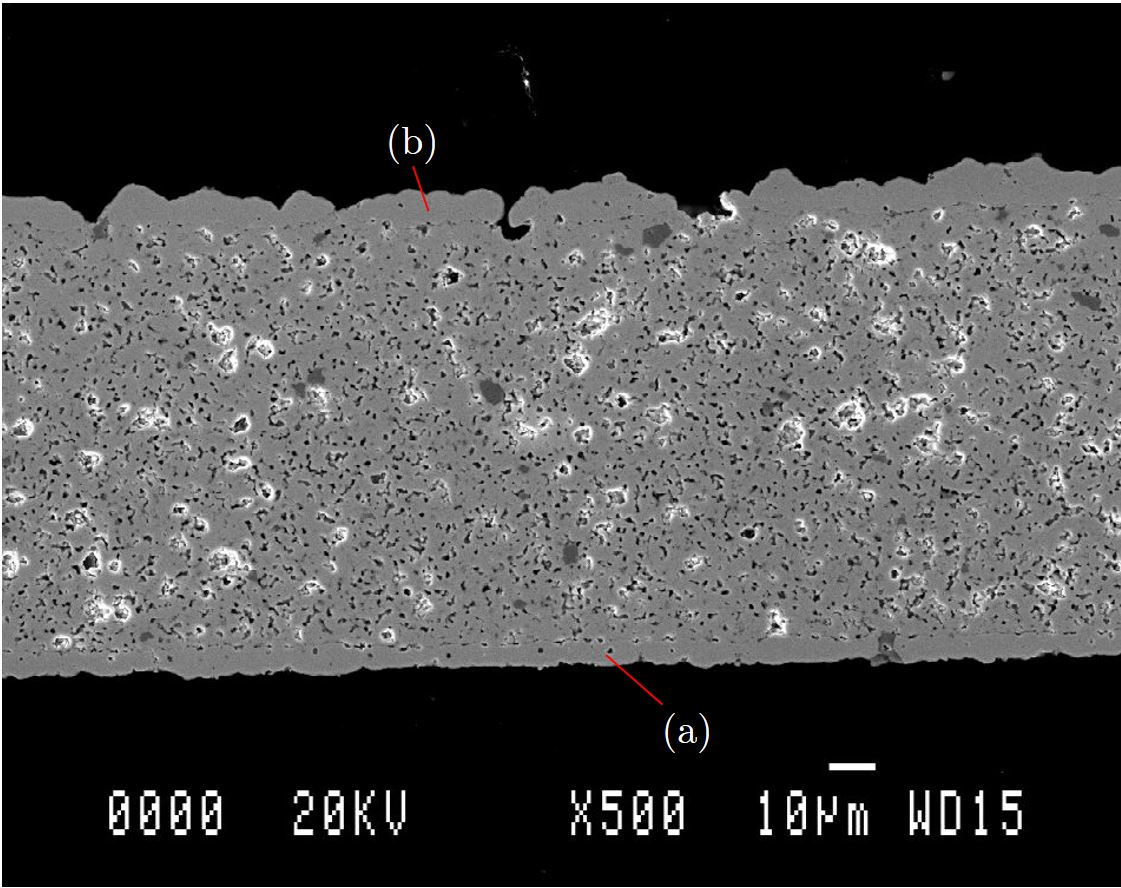
\includegraphics[width=\linewidth]{Images/agpd_ok_note.jpg}
%\subcaption{Double couche d'argent.}
%\label{agpd_ok}
%\end{subfigure}
%\caption{Microsections de micropoutres avec �lectrodes d'argent (i) simple couche et (ii) double couches vues au microscope �lectronique (�lectrons secondaires). Dans l'image (i) les �lectrodes (a) sup�rieure et (b) inf�rieure sont tr�s fines et totalement discontinues contrairement � l'image (ii).}
%\label{agpd}
\end{figure}



\section{Jonction plot-couche sacrificielle}
\label{pb_gap}
\subsection{�paisseur plot/couche sacrificielle}
La jonction entre le plot et la couche sacrificielle est critique a plusieurs titres. La jonction de la couche sacrificielle avec le plot impose que les couches aient la m�me hauteur pour que les couches ult�rieures s'impriment correctement et pour qu'elles ne pr�sentent pas de faiblesse structurelle trop importante. Une couche trop fine (Figure \ref{defects_CS}.\subref{profilo_244t_thin}) ou trop �paisse (Figure \ref{defects_CS}.\subref{profilo_244t_thick}) peut engendrer une cassure de la partie lib�r�e ou une discontinuit� de l'�lectrode inf�rieure.\\

\subsection{Alignement plot/couche sacrificielle}
L'alignement entre le plot et la couche sacrificielle est �galement critique. Un espace (�gap�) (Figure \ref{defects_CS}.\subref{profilo_244t_gap}) ou un trop grand recouvrement entre le plot et la couche sacrificielle peut engendrer une discontinuit� de l'�lectrode inf�rieure et �galement mener � la rupture de la partie lib�r�e.  Or, En raison des effets de bords des encres de s�rigraphie, i.e. la tendance qu'ont les motifs imprim�s � s'arrondir aux angles, une d�position exactement � la limite du plot n'est dans les faits pas possible. La couche sacrificielle s'arr�te soit juste avant le plot, l'arrondis en �paisseur cr�ant \textit{de facto} un gap, soit en contact avec le plot, le recouvrant alors l�g�rement. Ce dernier cas s'av�re le moins dommageable exp�rimentalement, ne donnant pas lieu � des d�faillances majeures.\\

\begin{figure}
\begin{subfigure}[t]{0.3\textwidth}
\centering
\begin{tikzpicture}[scale=0.75]
\begin{axis}[
	mark size=0,
	line width = 1,
	ticks = none]
\addplot table [y=Y, x=X]{Images/Al2O3_plot_PZT_244t_2_layers_244T_1.dat};
\addplot table [y=Y, x=X]{Images/Al2O3_plot_PZT_244t_2_layers_244T_2.dat};
\end{axis}
\end{tikzpicture}
\caption{Trop fine}
\label{profilo_244t_thin}
\end{subfigure}
~
\begin{subfigure}[t]{0.3\textwidth}
\centering
\begin{tikzpicture}[scale=0.75]
\begin{axis}[
	mark size=0,
	line width = 1,
	ticks = none]
\addplot table [y=Y, x=X]{Images/Al2O3_plot_PZT_244t_3_layers_244T_ter_1.dat};
\addplot table [y=Y, x=X]{Images/Al2O3_plot_PZT_244t_3_layers_244T_ter_2.dat};
\end{axis}
\end{tikzpicture}
\caption{Trop �paisse}
\label{profilo_244t_thick}
\end{subfigure}
~
\begin{subfigure}[t]{0.3\textwidth}
\centering
\begin{tikzpicture}[scale=0.75]
\begin{axis}[
	mark size=0,
	line width = 1,
	ticks = none]
\addplot table [y=Y, x=X]{Images/Al2O3_plot_PZT_244t_3_layers_244T_1.dat};
\addplot table [y=Y, x=X]{Images/Al2O3_plot_PZT_244t_3_layers_244T_2.dat};
\end{axis}
\end{tikzpicture}
\caption{Gap}
\label{profilo_244t_gap}
\end{subfigure}
\caption{Profilographes de diff�rents d�fauts d'impression de la couche sacrificielle. ({\color{blue} �} plot, {\color{red} �} couche sacrificielle).}
\label{defects_CS}
\end{figure}

\subsection{Ordre et direction d'impression}
Pour l'obtention d'un l�ger recouvrement plot/couche sacrificielle, l'ordre d'impression d�finit quelle couche recouvre l'autre. Si la couche sacrificielle est imprim�e en premier, le plot est imprim� de fa�on � l�g�rement recouvrir la couche sacrificielle. Si cela ne change pas les �tapes d'impression ult�rieures, la partie lib�r�e se r�v�le fragilis�e et casse lors de la lib�ration durant le frittage. La couche sacrificielle est donc imprim�e apr�s le plot de fa�on � l�g�rement la recouvrir, ce qui permet la lib�ration des micropoutres sans fracture. La Figure \ref{jonction} illustre �galement le probl�me de la direction d'impression. 

\begin{figure}
\centering
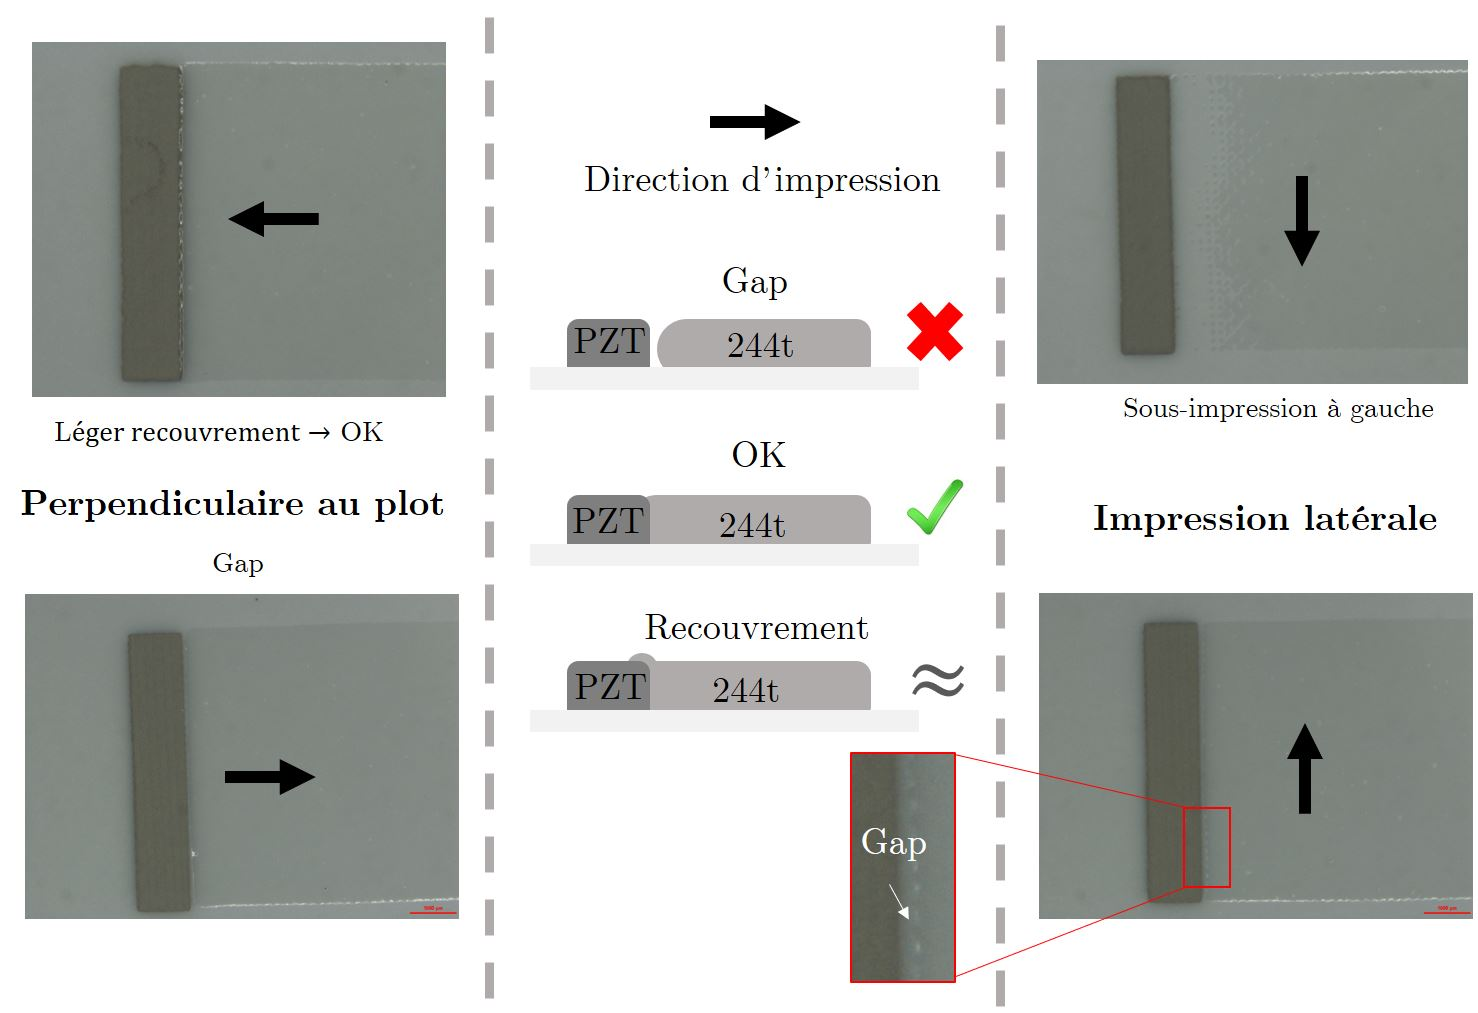
\includegraphics[width=\linewidth]{Images/jonction.jpg}
\caption{Illustration des diff�rents d�fauts rencontr�s � la jonction en fonction de la direction d'impression. Dans cet exemple, la couche sacrificielle est imprim�e apr�s le plot. Un recouvrement partiel est tol�rable (�{\color{gray}\Large{$\approx$}}�) dans ce cas pr�cis car bien plus facile � r�aliser et sans grandes cons�quences pour le reste du proc�d�, ce qui pourrait ne pas �tre le cas dans un autre proc�d�.}
\label{jonction}
\end{figure}


\section{Frittage et polarisation}
\subsection{Frittage}
\subsubsection{Profil utilis�}
L'ensemble des couches est fritt� � 900�C pendant 2 heures dans un four vertical � passage selon le profil de temp�rature indiqu� Figure \ref{profil_frittage}. Les �chantillons sont chauff�s avec un gradient de 40�C/min jusqu'� 250�C. On utilise ensuite un r�gime lent de mont�e en temp�rature entre 250�C et 450�C � 1�C/min, pendant la d�composition des liants organiques et de la couche sacrificielle. Un gradient de 40�C/min est � nouveau utilis� jusqu'� 900�C. S'ensuit  un plateau de 2h � 900�C, puis une descente rapide � 40�C/min jusqu'� environ 150�C, o� les �chantillons sont ensuite refroidis par l'environnement � temp�rature ambiante. L'utilisation de l'aide au frittage LBCu permet un frittage du PZT � 900�C \cite{Medesi2014}. Le Tableau \ref{frittage} donne les �paisseurs des couches apr�s frittage. On observe une certaine dispersion des �paisseurs d'un lot � l'autre.\\

\begin{table}
\centering
\caption{Tableau des �paisseurs des diff�rentes couches apr�s �tuvage ($h_{etu.}$) et apr�s frittage ($h_{fritt.}$).}
\label{frittage}
\begin{tabular}{|c|c|c|c|}\hline
Couche							&Encre							&$h_{etu.}$ (\textmu m)	&$h_{fritt.}$ (\textmu m)\\\hline\hline
Plot								&PZT								&30-40									&25-30\\\hline
Coucre sacricielle	&ESL244t (polyester)&30-40									&-\\\hline
�lectrode inf�rieure&ESL8836 (or)				&15											&10-15\\\hline
Partie lib�r�e			&PZT								&100-120								&80-100\\\hline
�lectrode sup�rieure&ESL8836 (or)				&8											&5-8\\\hline
\end{tabular}
\end{table}





\subsubsection{�vaporation de PbO}
Le monoxyde de plomb PbO est un compos� dont la temp�rature d'�bullition se trouve proche de 900�C et qui � �tre volatile durant le frittage du PZT. Pour �viter de trop grandes pertes en plomb dans la composition du PZT durant le frittage, des couvercles sont pos�s pour confiner l�atmosph�re autour des �chantillons. Il est �galement possible d'ajouter des compos�s du plomb en sus des �chantillons pour saturer d'avantage l'atmosph�re en PbO et ainsi limiter son �vaporation depuis le PZT \cite{Safar2017}. Un des sympt�mes d'une �vaporation importante de PbO depuis le PZT est l'apparition de domaines d'oxyde de zirconium ZrO$_2$. On rapporte dans la litt�rature une diminution de la densit� et des propri�t�s �lectrom�caniques  par rapport � un PZT �quilibr� ou m�me en exc�s de PbO \cite{Kingon1983, Garg1999}. Si peu ou pas de domaines ne sont  observ�s sur des �chantillons fritt�s � 900�C, plusieurs frittages effectu�s � 930�C mettent en �vidence l'importance du ph�nom�ne d'�vaporation du PbO � partir du PZT. Sur la Figure \ref{PbO_evap} on observe clairement des domaines plus sombres dans le PZT fritt� � 930�C, absents de celui fritt� � 900�C. Une analyse aux rayons X confirme qu'il s'agit bien de ZrO$_2$.\\ 

\begin{figure}
\centering
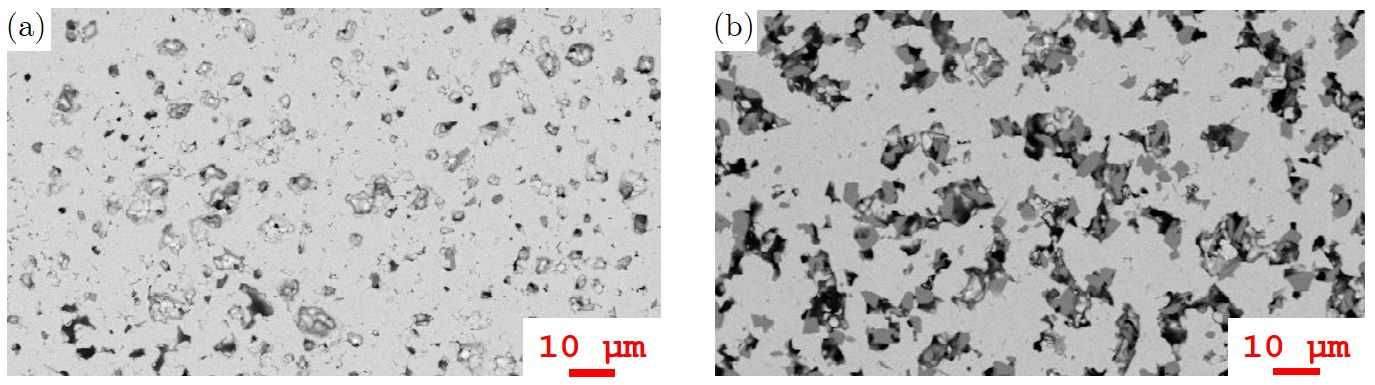
\includegraphics[width=0.8\linewidth]{Images/PbO_evap.jpg}
\caption{Image MEB (r�trodiffusion d'�lectrons) (a) du PZT d'un �chantillon fritt� � 900�C et (b) d'un autre �chantillon fritt� � 930�C. Les t�ches sombres sur l'image (b) sont des domaines de dioxyde de zirconium.}
\label{PbO_evap}
\end{figure}

\begin{figure}
\centering
\begin{tikzpicture}
\begin{axis}[
  xlabel=Temps (s),
  ylabel=Temp�rature (�C),
	%minor xtick={0,25,...,200},
	%minor ytick={0,50,...,400},
	mark size = 0,
	line width = 1,
	grid=major]
	%legend cell align={left},
	%legend style={at={(0.03,0.5)},anchor=west}]
%\draw[step=1cm,gray,very thin] (-2,-2) grid (6,6);	
\addplot table [y=Consigne, x=Temps,dotted]{Images/frittage.dat};
%\addlegendentry{Consigne}
\addplot table [y=Mesure, x=Temps]{Images/frittage.dat};
%\addlegendentry{Temp�rature �chantillon}
\end{axis}
\end{tikzpicture}
\caption{Profil de frittage utilis� avec les encres PZT non broy�es. ({\color{blue} �} Consigne, {\color{red} �} Temp�rature �chantillon)}
\label{profil_frittage}
\end{figure}


\subsection{Polarisation}
\subsubsection{Principe}
La polarisation du PZT consiste � aligner les domaines ferro�lectriques internes � l'aide d'un champ magn�tique et d'une �l�vation de la temp�rature au dessus de la temp�rature de Curie. La temp�rature de Curie est la temp�rature � partir de laquelle les domaines deviennent mobiles, permettant ainsi la polarisation et la conservation de cette derni�re une fois la temp�rature descendu en dessous. Les micropoutres sont polaris�es dans un four de polarisation en atmosph�re inerte � 280�C sous un champ �lectrique de 3 kV/mm pendant 5 min. 

\subsubsection{Am�liorations apport�es}
Une cellule de polarisation est d�velopp�e pour assurer la connexion entre les alimentations �lectriques et les micropoutres (voir Figure \ref{module_pola}). Les micropoutres peuvent �galement �tre connect�es via des fils d'argents coll�s sur les �lectrodes avec une p�te argent-�poxy. Le module permet de s'affranchir de l'�tape de collage des fils et ne souffre pas de vieillissement thermique contrairement � la p�te argent-�poxy.

\begin{figure}
\centering
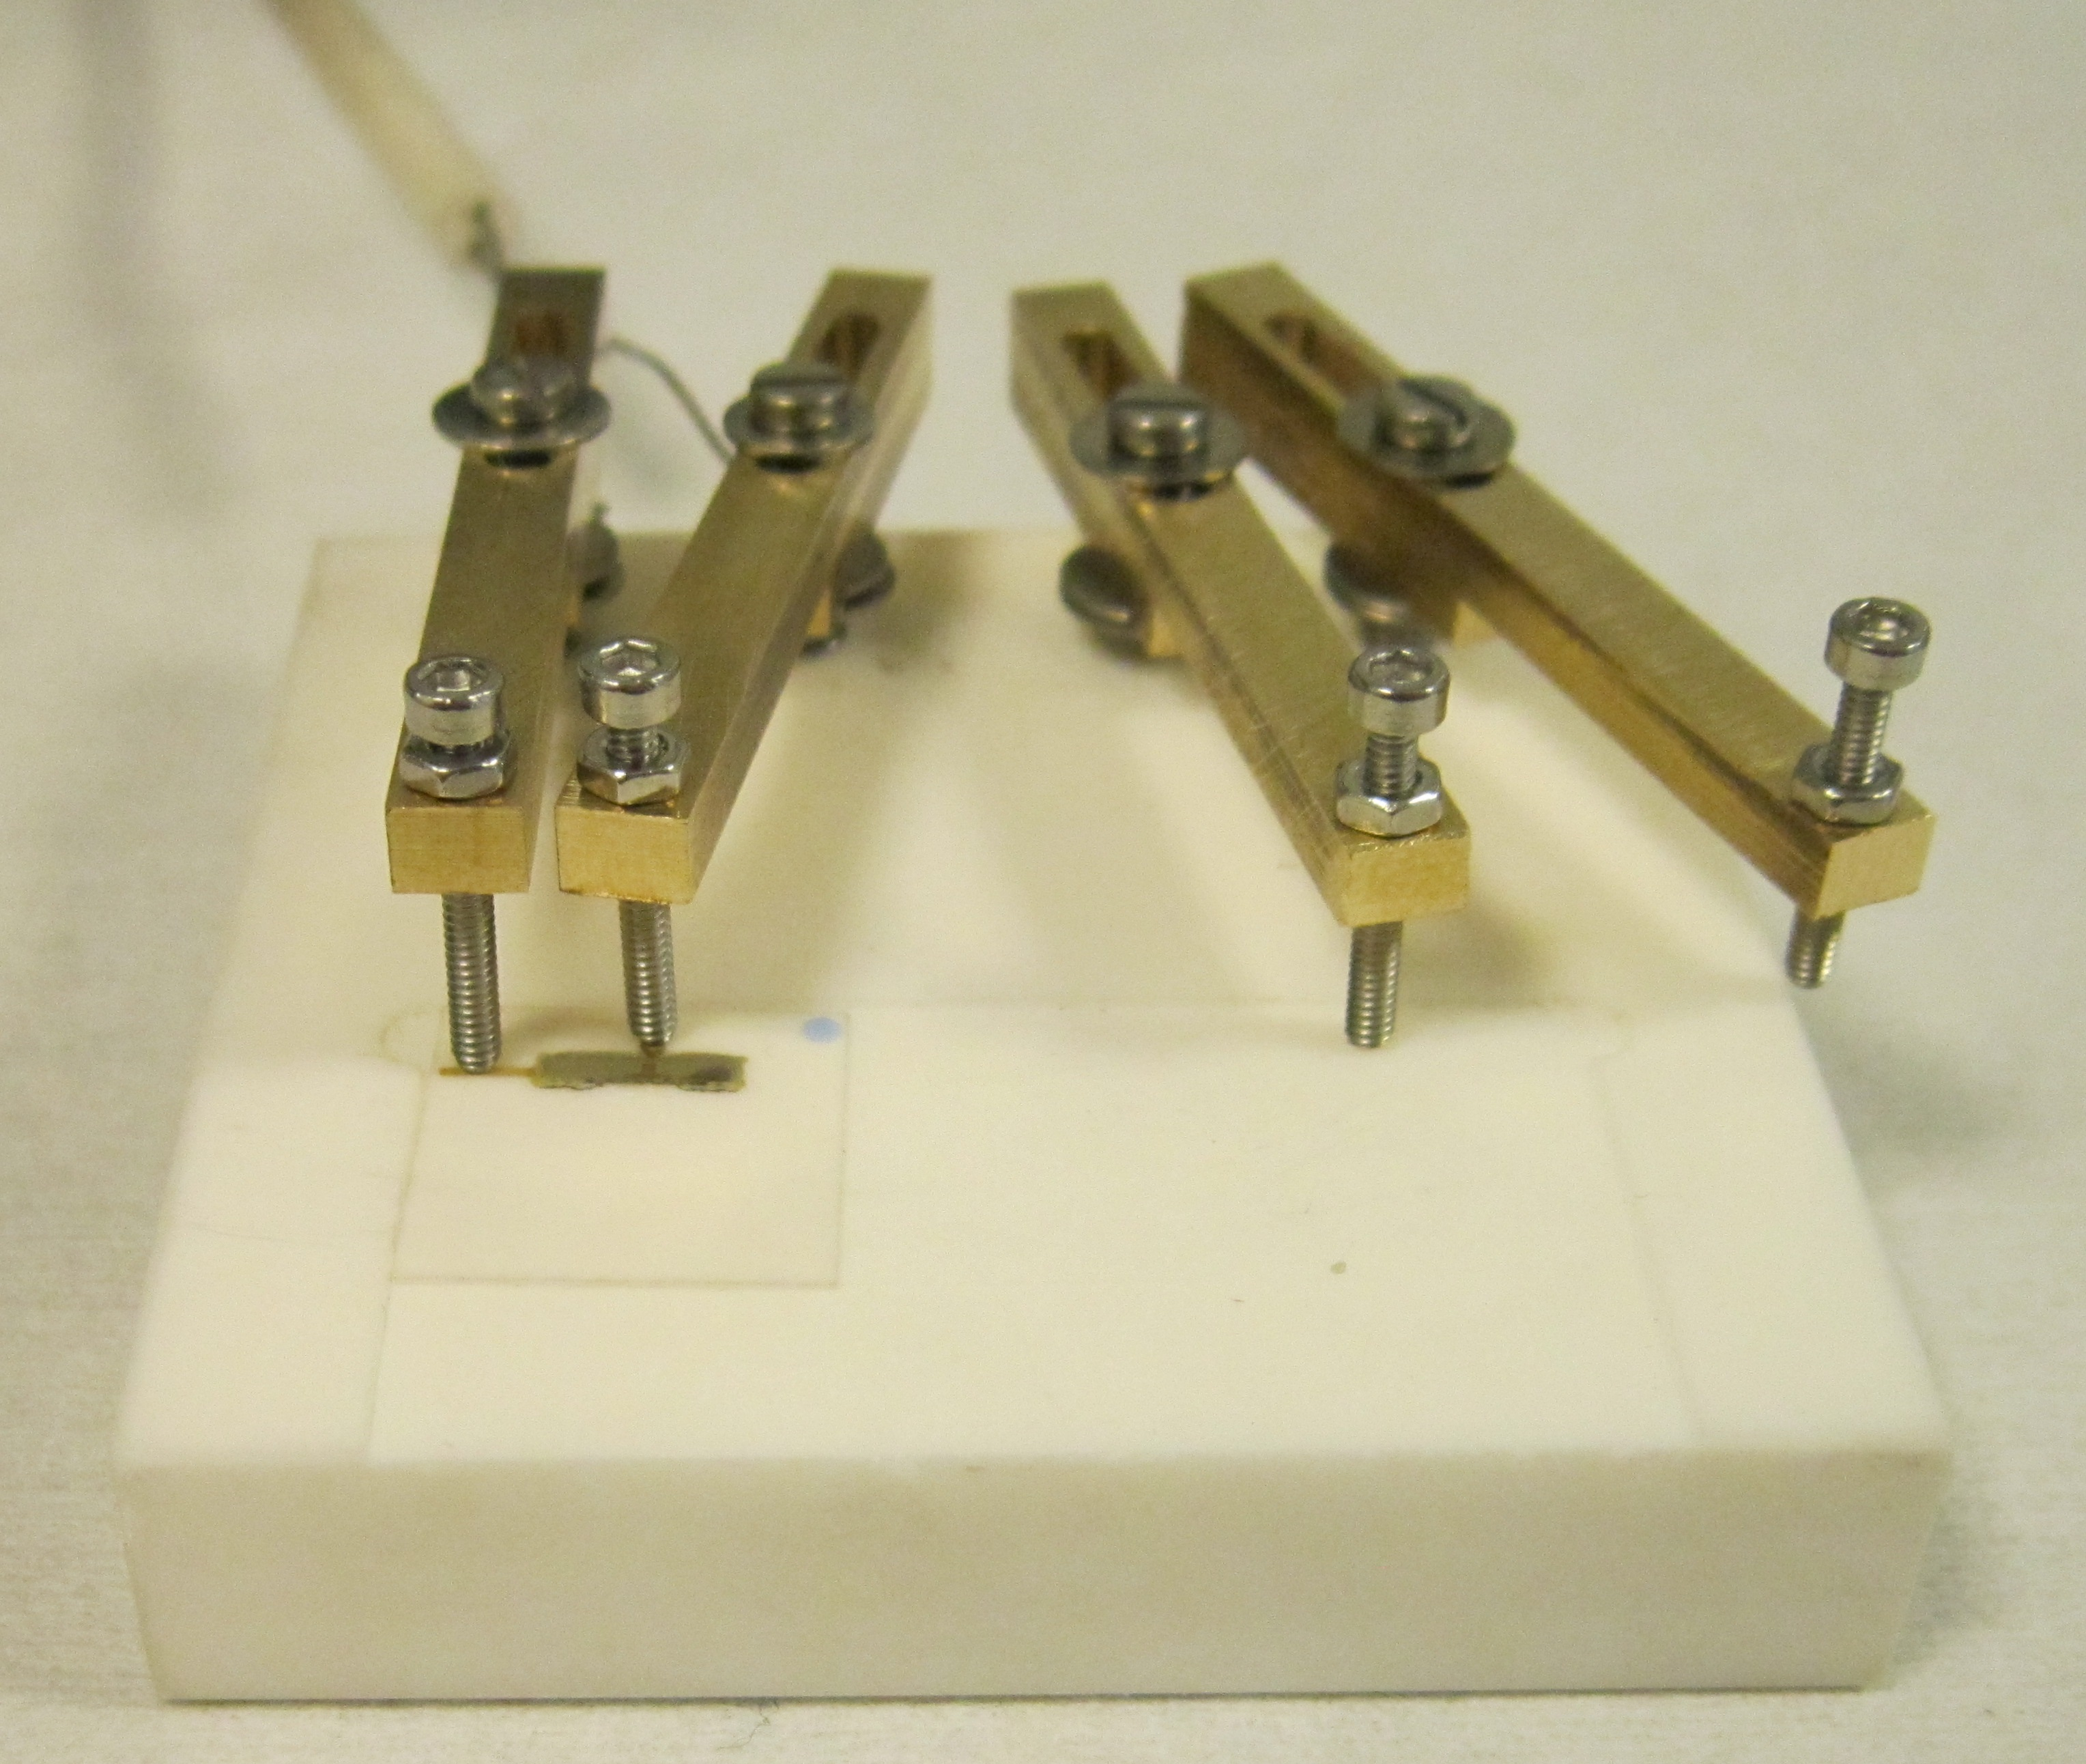
\includegraphics[width=0.6\linewidth]{Images/module_pola.jpg}
\caption{Photo du dispositif utilis� pour la connexion des micropoutres aux alimentation �lectriques lors de la polarisation. Les contacts sont en acier et les bras mobiles en laiton. Les bras sont mont�s sur ressorts et peuvent s'adapter � plusieurs formes d'�chantillons et d'�lectrodes. Le socle est r�alis� en c�ramique usinable au sein du laboratoire (Macor\textregistered, Final Advanced Ceramics). En arri�re plan, on peut voir une gaine en c�ramique et deux fils de platine coinc�s sous les bras par des rondelles. Ils connectent la cellule aux alimentations �lectriques.}
\label{module_pola}
\end{figure}

\section{Interactions entre les couches}
\subsection{PZT broy� : fissures dans l'�lectrode sup�rieure}
Une cons�quence non-d�sir�e de l'utilisation de PZT broy� est l'apparition de fissures sur l��lectrode sup�rieure apr�s frittage qui coupent l'�lectrode en deux entre la zone active et la zone de contact (voir Figure \ref{ES_crack}). Deux strat�gies sont utilis�es pour tenter d'�viter le probl�me en jouant sur la composition de l'�lectrode sup�rieure et le profil de frittage .
\begin{figure}
\centering
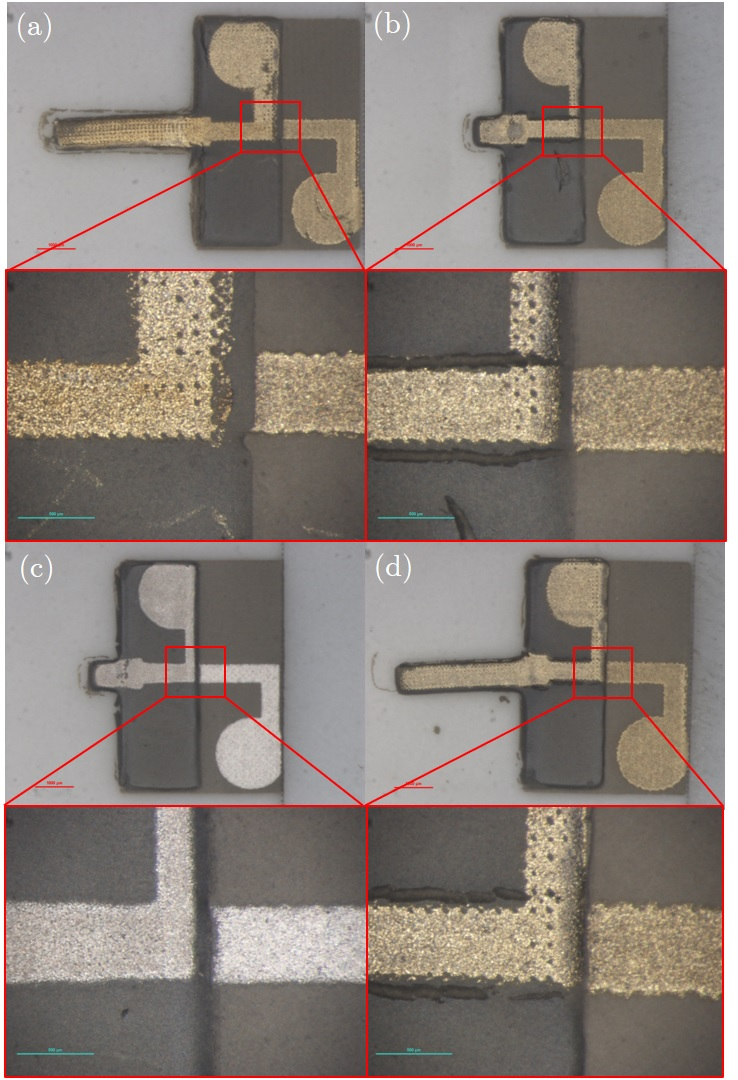
\includegraphics[height=0.8\textheight]{Images/ES_cracks.jpg}
\caption{(a) Image optique d'une micropoutre avec �lectrode d'or et encre PZT non broy�e. Aucune fissure n'est visible sur la partie zoom�e. (b) Micropoutre avec �lectrode d'or et encre PZT broy�e. Des fissures sont visibles sur la partie zoom�e et coupent l'�lectrode sup�rieure. (c) Micropoutre avec �lectrode en argent palladium et encre PZT broy�e. Aucune fissure n'est visible sur la partie zoom�e. (d) Micropoutre avec �lectrode d'or et encre PZT broy�e fritt�e avec le profil lent (Figure \ref{profil_frittage_broyees}). Des fissures sont visibles sur la partie zoom�e mais sont arr�t�es par l'�lectrode sup�rieure.}
\label{ES_crack}
\end{figure}

\subsubsection{Adaptation des compositions d'encres}
L'encre � base d'argent d�crite pr�c�demment section \ref{AgPd} ne pr�sente pas de fissure lorsque utilis�e avec le PZT broy�, et ce quelques soit le frittage utilis� (voir Figure \ref{ES_crack} (c)). La partie min�rale de l'encre argent diff�re de celle pr�sente dans l'encre d'or, d�termin�e dans une �tude pr�c�dente � la microsonde Castaing \cite{Lakhmi2011}. Le Tableau \ref{compo_mineral} recense les compos�s pr�sents dans les encres. \\
Cependant, les essais de polarisations et caract�risations ult�rieures montrent que les micropoutres avec les �lectrodes en argent claquent souvent � tr�s faibles tension, emp�chant leur polarisation et les rendant donc inexploitables pour la plupart. Une solution serait d'adapter l'encre d'or avec les ajouts de la phase min�rale utilis�e dans l'encre d'argent, ou de modifier ces ajouts pour rendre l'encre d'argent compatible  avec la polarisation des micropoutres. (Attente infos TEMEX)


\begin{table}
\caption{Composition min�rale des encres. �\textepsilon� indique des traces de l'�l�ment en question.}
\label{compo_mineral}
\vspace{0.4cm}
\centering
\begin{tabular}{|c||c|c|c|c|c|c|c|c|c|}
\hline
\% molaire 	&SiO$_2$	&Al$_2$O$_3$&CaO	&Bi$_2$O$_3$&Au	&CdO	&PbO	&Ag	&Pd	\\\hline\hline
Au ESL8836 	&4,6			&1,7				&0,9	&1,2				&84	&2,7	&4,8	&0	&0	\\\hline
AgPd TEMEX	&-				&-					&-		&-					&-	&-		&-		&-	&-	\\\hline
\end{tabular}
\end{table}



\subsubsection{Adaptation du profil de frittage au PZT broy�}

L'utilisation de PZT broy� entra�ne l'augmentation du retrait apr�s le frittage. Il s'agit ici de probl�me de compatibilit� de coefficients de retrait thermique  et des fissures que cela cr�e dans les �lectrodes. Une solution (partielle) est d'adapter le profil de temp�rature pour essayer de rendre moins brutale le retrait du PZT vis-�-vis des autres couches. Le profil est donc adapt� avec une mont�e � 1�C/min entre 250�C et 900�C (Figure \ref{profil_frittage_broyees}). La Figure \ref{ES_crack} illustre les diff�rences entre micropoutres fabriqu�es avec une encre PZT non broy� (a), avec une encre PZT broy� (b) et avec une encre PZT broy� et fritt� avec le profil lent utilis� pour essayer de limiter les contraintes (et donc les fissures). Si dans le cas d'un frittage classique avec encre PZT broy� les fissures rendent la quasi-totalit� des micropoutres inutilisables, le frittage lent limite l'�tendue des fissures qui he coupent pas l'�lectrode sup�rieure (Figure \ref{ES_crack} (d).

\begin{figure}
\centering
\begin{tikzpicture}
\begin{axis}[
  xlabel=Temps (s),
  ylabel=Temp�rature (�C),
	%minor xtick={0,25,...,200},
	%minor ytick={0,50,...,400},
	mark size = 0,
	line width = 1,
	grid=major]
	%legend cell align={left},
	%legend style={at={(0.03,0.5)},anchor=west}]
%\draw[step=1cm,gray,very thin] (-2,-2) grid (6,6);	
\addplot table [y=Consigne, x=Temps,dotted]{Images/frittage_milled.dat};
%\addlegendentry{Consigne}
\addplot table [y=Mesure, x=Temps]{Images/frittage_milled.dat};
%\addlegendentry{Temp�rature �chantillon}
\end{axis}
\end{tikzpicture}
\caption{Profil de frittage utilis� avec les encres PZT broy�es.. ({\color{blue} �} Consigne, {\color{red} �} Temp�rature �chantillon)}
\label{profil_frittage_broyees}
\end{figure}

En attente
(Une encre � base d'argent-palladium dont la fritte de verre serait adapt�e aux conditions de frittage et a l'application r�sonateur PZT, i.e. sans int�ractions d�gradants le)


\subsection{Solvants et couche sacrificielle}
\label{inter_solvants}
Pour les �lectrodes d'or (ESL 8836), on observe une d�gradation notable de l'�lectrode inf�rieure par rapport � la sup�rieure lorsque une seule couche est s�rigraphi�e, comme montr� sur l'image MEB Figure \ref{MEB_bad_EI}. Une solution est d'imprimer une couche plus �paisse d'or pour l'�lectrode inf�rieure. La Figure \ref{MEB_good_EI} montre une �lectrode inf�rieure l�g�rement poreuse mais continue. L'�lectrode inf�rieure est imprim�e en deux fois pour une �paisseur s�che de 15 \textmu m, l'�lectrode sup�rieure est imprim�e en une fois, pour une �paisseur s�che de 8 \textmu m.\\
Cette interaction est probablement une interaction li�e aux solvants en pr�sence (voir Figure \ref{solvants}) que sont le terpin�ol dans la couche d'or et l'ac�tate de butyle diglycol dans la couche sacrificielle 244t, tous deux polaires. En effet, la d�gradation n'est pas observ�e avec l'encre � base d'argent dont le solvant NOM SOLVANT est aliphatique, i.e. non polaire et donc non miscible avec le solvant de la 244t.

\begin{figure}
\centering
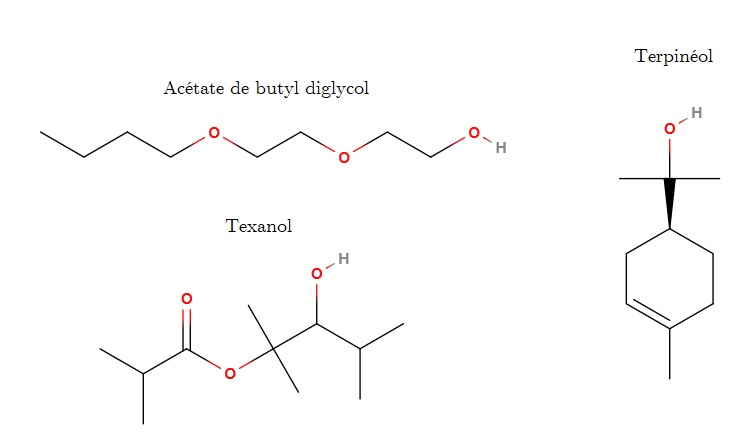
\includegraphics[width=0.8\linewidth]{Images/solvants.jpg}
\caption{Formules chimique du Terpin�ol, solvant des encres d'or ESL8836, du Texanol, solvant inclus dans le v�hicule ESL V400 des encres PZT, et de l'ac�tate de butyl diglycol, inclus dans le v�hicule ESL CV59 des encres SrCO$_3$ et farine de ma�s ainsi que dans l'encre polyester ESL 244t.}
\label{solvants}
\end{figure}


\begin{figure}
\centering
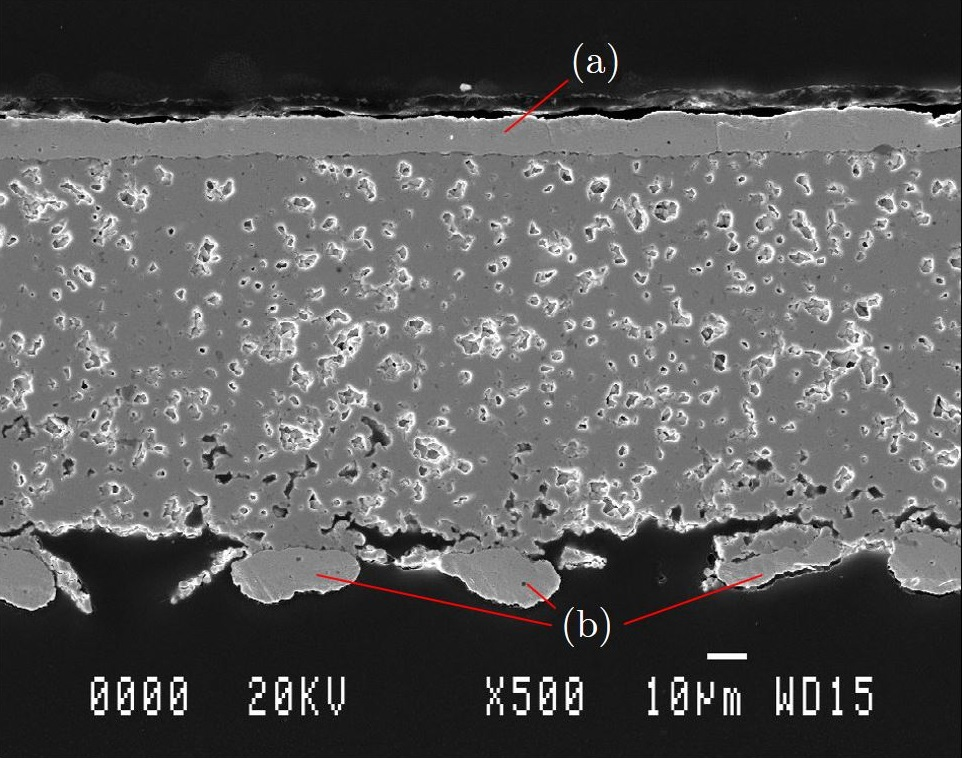
\includegraphics[width=0.6\linewidth]{Images/MEB_bad_EI_note.jpg}
\caption{Microsection d'une micropoutre avec �lectrodes d'or simples vue au microscope �lectronique. (a) L'�lectrode sup�rieure et (b) inf�rieure apparaissent plus claires de par et d'autre de la partie poreuse centrale en PZT. On observe clairement une d�gradation de l'�lectrode inf�rieure par rapport � la sup�rieure.}
\label{MEB_bad_EI}
\end{figure}

\begin{figure}
\centering
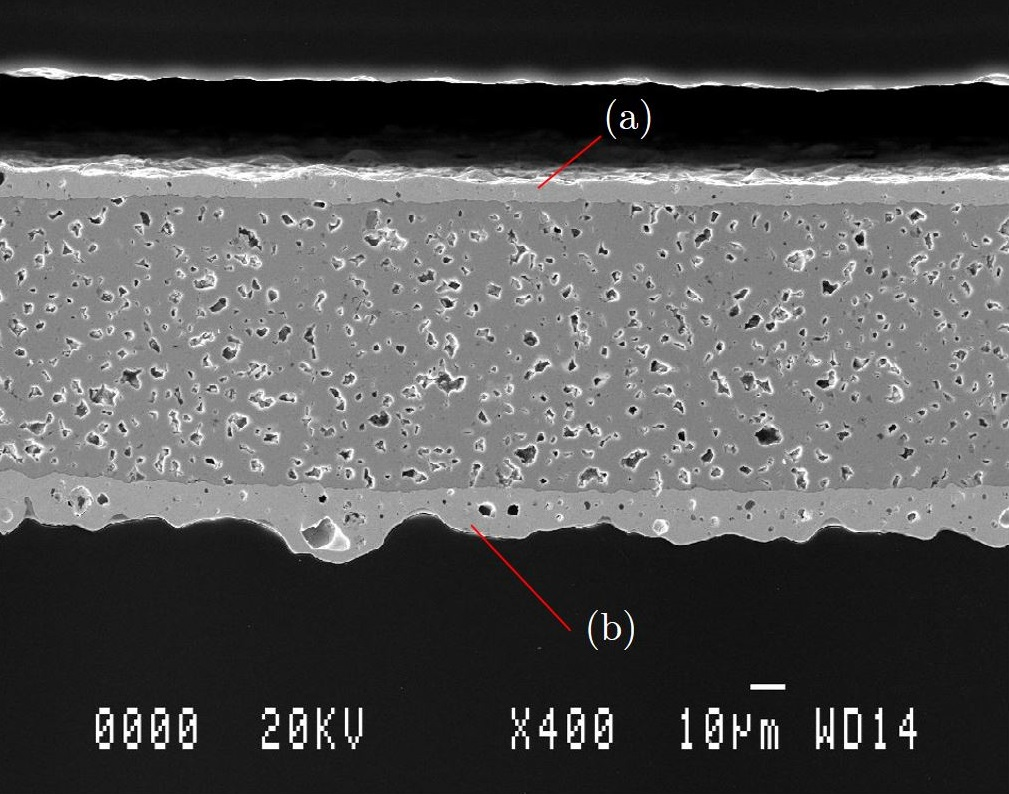
\includegraphics[width=0.6\linewidth]{Images/MEB_good_EI_note.jpg}
\caption{Microsection d'une micropoutre avec �lectrodes d'or vue au microscope �lectronique. (a) L'�lectrode sup�rieure est imprim�e en une fois alors que (b) l'�lectrode inf�rieure l'est en deux fois et est donc plus �paisse. Si l'�lectrode inf�rieure semble d�grad�e elle n'en reste pas moins continue.}
\label{MEB_good_EI}
\end{figure}







\section{Densification}\label{carac}
\subsection{Porosit� et masse volumique}
La porosit� des �chantillons est estim�e de 2 fa�ons :
\begin{itemize}
\item par  analyse num�rique de microsections observ�es au microscope �lectronique (MEB),
\item par pycnom�trie gazeuse.
\end{itemize}

L'analyse num�rique d'images MEB consiste � compter les trous observables sur une microsection plane et calculer leur surface cumul�e. Le proc�d� peut �tre fait � l'aide de logiciels gratuits tel que ImageJ. Le ratio de la surface de trous sur la surface totale observ�e permet une estimation du pourcentage de porosit� dans le solide. Cette m�thode est approximative pour deux raisons : on peut se tromper dans l'identification de ce qu'est un trou et on ne regarde le solide que sur un plan, celui de la microsection. La valeur de $\rho_{ref.}$ = 7700 kg/m$�$ est choisie comme valeur de r�f�rence pour la masse volumique du PZT (non poreux). On peut faire une estimation de la densit� du PZT des micropoutres observ�es a partir de cette valeur : $\rho = (1-$\emph{porosit�}$)*\rho_{ref.}$\\ 
La pycnom�trie permet de conna�tre le volume d'un solide poreux avec une grande pr�cision (� condition que la porosit� soit ouverte) en utilisant le volume occup� par un gaz (helium en g�n�ral) dans une chambre de r�f�rence � une pression donn�e et le volume et la pression de ce m�me gaz dans une chambre contenant l'�chantillon.\\ 

Le Tableau \ref{porosite} montre les r�sultats des estimations de la masse volumique de la partie lib�r�e et de disques de PZT. On note une nette augmentation de la masse volumique entre couches sacrificielles SrCO$_3$ et 244t. Ceci peut s'expliquer par la pr�sence de poudre min�rale jusqu'� la fin du frittage pour la couche SrCO$_3$, pouvant freiner la densification du PZT en retenant la partie lib�r�e. On observe une densification comparables entre les micropoutres fabriqu�es sur 244t et sur couche sacrificielle de ma�s, cette derni�re permettant m�me une meilleure densification pour les disques.Enfin, le PZT broy� permet bien d'augmenter la masse volumique et ce quelles que soient les conditions de fabrication.\\
L'int�r�t d'avoir une meilleure densification est multiple :
\begin{itemize}[label=$\bullet$]
\item meilleure tenue m�canique
\item meilleure propri�t�s �lectrom�caniques, du fait du moins grand nombre de cavit�s assimilables � des d�fauts
\item fr�quence de r�sonance plus �lev�e, du fait du raccourcissement des micropoutres, qui permet en th�orie d'atteindre des sensibilit�s plus  �lev�es
\end{itemize}

\begin{table}
\caption{Estimations de la masse volumique $\rho$ de la partie lib�r�e des micropoutres et de disques. La porosit� est estim�e uniquement via analyse d'image MEB. }
\label{porosite}
\vspace{0.4cm}
\centering
\begin{tabular}{|c|c|c|c|c|c|}
\hline
\multirow{2}{*}{Type d'�chantillon}	&\multirow{2}{*}{PZT}				&Couche								&\multirow{2}{*}{Porosit� (\%)}					&\multicolumn{2}{c|}{$\rho$ (kg/m$�$)}		\\\cline{5-6}
																		&														&sacrificielle				&																				&Analyse MEB	&Pycnom�trie		\\\hline\hline
																		
\multirow{4}{*}{Micropoutres}				&\multirow{2}{*}{Non broy�}	&SrCO$_3$							&31,2$\pm$3,4														&5300$\pm$260 &-							\\\cline{3-6}
																		&														&244t									&12,7$\pm$1,5														&6720$\pm$120	&6790						\\\cline{2-6}
																		&\multirow{2}{*}{Broy�}			&244t									&6,2$\pm$1,7														&7200$\pm$130	&-							\\\cline{3-6}
																		&														&Ma�s									&6,7$\pm$1,5														&7180$\pm$120	&-							\\\hline
\multirow{3}{*}{Disques}						&Non broy�									&244t\footnotemark[1]	&	-																			&-						&-							\\\cline{2-6}
																		&\multirow{2}{*}{Broy�}			&244t\footnotemark[1]	&6,7$\pm$1,5														&7180$\pm$120	&-							\\\cline{3-6}
																		&														&Ma�s									&2,2$\pm$0,4														&7530$\pm$30	&-							\\\hline
																		
\end{tabular}
\end{table}
\footnotetext[1]{Disques fabriqu�s par Onuma Santawitee (liens Article/Th�se � venir)}


\subsection{Retrait longitudinal}
Le retrait longitudinal est une autre fa�on d'observer la densification en mesurant la longueur des micropoutres avant et apr�s le frittage. Les r�sultats sont rassembl�s dans le Tableau \ref{retrait} et la Figure \ref{retrait_plot}. Le retrait a tendance � augmenter quand la longueur diminue. L'incertitude augmente �galement avec la longueur, ceci principalement en raison de l'augmentation de l'importance de l'erreur de mesure relative avec la diminution de la longueur. Mais m�me en prenant en compte cette incertitude, la tendance est nette que ce soit des poutres imprim�es avec un PZT broy� ou non. Ceci peut �tre d� � la plus faible surface � lib�rer qui a d�s lors plus de libert� pour se densifier.\\

\begin{table}
\centering
\caption{Tableau des retraits moyens observ�s en fonction du type d'encre PZT et des dimensions des micropoutres. Toutes les micropoutres sont imprim�es et lib�r�es avec la couche sacrificielle 244t. Un minimum de 4 micropoutres est imprim� pour chaque valeur moyenne indiqu�e.}
\label{retrait}
\begin{tabular}{|c|c|c|c|}\hline
\multirow{2}{*}{$L$ (mm)}&\multirow{2}{*}{$w$ (mm)}	&\multicolumn{2}{c|}{Retrait (\%)}	\\\cline{3-4}
												&													&PZT broy�		&PZT non broy�					\\\hline\hline														
8												&2												&15,7$\pm$1,5	&12,9$\pm$1,4						\\\hline
8												&1												&-						&-											\\\hline
4												&2												&16,6$\pm$2,1	&13,6$\pm$1,9						\\\hline
4												&1												&18,1$\pm$2,8	&12,7$\pm$1,9						\\\hline
2												&2												&25,7$\pm$7,9	&17,9$\pm$3,1						\\\hline
2												&1												&20,3$\pm$2,0	&17,5$\pm$2,4						\\\hline
1												&2												&28,9$\pm$9,5	&26,2$\pm$2,8						\\\hline
1												&1												&25,9$\pm$4,0	&24,1$\pm$3,3						\\\hline
\end{tabular}
\end{table}

\begin{figure}
\centering
\begin{tikzpicture}[scale=1] 
\begin{axis} [
symbolic x coords={8x2,4x2,4x1,2x2,2x1,1x2,1x1},
xtick=data,
minor ytick={0.10,0.125,...,0.40},
xlabel = $L\times w$,
ylabel = Retrait,
scaled ticks=false,
yticklabel=\pgfmathparse{100*\tick}\pgfmathprintnumber{\pgfmathresult}\,\%,
yticklabel style={/pgf/number format/.cd,fixed,precision=2},
legend cell align={left},
legend style={at={(0.03,0.87)},anchor=west},
grid=minor]

\addplot+[only marks] 
  plot[error bars/.cd, y dir=both, y explicit]
  table[x=L,y=Non_broye,y error plus expr=\thisrow{STD1},y error minus expr=\thisrow{STD1}] {Images/retrait.dat};\addlegendentry{Non broy�}

\addplot+[only marks] 
  plot[error bars/.cd, y dir=both, y explicit]
  table[x=L,y=broye,y error plus expr=\thisrow{STD2},y error minus expr=\thisrow{STD2}] {Images/retrait.dat};\addlegendentry{Broy�}

\end{axis} 
\end{tikzpicture}
\caption{Valeurs moyennes et �carts-type des retraits observ�s pour diff�rentes g�om�tries.}
\label{retrait_plot}

\end{figure}
\section{Conclusion}



\bibliographystyle{unsrt}
\bibliography{Fabrication_biblio}

\end{document}
%\cleardoublepage
%
%\input{M�thodes et caract�risations}
%\cleardoublepage
%
%\input{Exp�riences}
%\cleardoublepage
%
%\input{Conclusion}
%\cleardoublepage


\subsection{Comments}

Comments can be added to the margins of the document using the \todo{Here's a comment in the margin!} todo command, as shown in the example on the right. You can also add inline comments too:

\todo[inline, color=green!40]{This is an inline comment.}



%% Preamble______________________________________________________________________
%
%\pagenumbering{roman} 				% Begin roman page numbering (i,ii,...)
%
%\input{chapters/preamble}
%
%% Chapters______________________________________________________________________
%
%\pagestyle{fancy}               	% Fancy headings
%\pagenumbering{arabic}				% Begin arabic page numbering (1,2,...)
%
%\input{chapters/introduction}
%\cleardoublepage
%\input{chapters/howto}
%\cleardoublepage
%% \input{}
%% \cleardoublepage
%% \input{}
%% \cleardoublepage
%% ...
%
%% Appendix______________________________________________________________________
%\appendix
%\input{chapters/appendix}


% Bibliography__________________________________________________________________
% Literature (Additional references can be added to the .bib-file manually, or by using, for example, the free application JabRef). Compile in the following order: latex -bibtex -latex -latex
\end{document}